\documentclass[a4paper,12pt,titlepage]{report}
\bibliographystyle{styles/vancouver}
\usepackage{cite}
\usepackage{fullpage}
\usepackage{setspace}
\usepackage{graphics}
\usepackage{amstext}
\usepackage{amsmath}
\doublespacing


\newcommand{\unit}[2]{\ensuremath{#1\,\text{#2}}}
\newcommand{\cms}[1]{\ensuremath{#1\,\text{cms}^{\text{-1}}}}

\newcommand{\ms}[1]{\unit{#1}{ms}}
\newcommand{\msrange}[2]{\ensuremath{#1\text{--}#2\,\text{ms}}}
\newcommand{\mm}[1]{\unit{#1}{mm}}
\newcommand{\mv}[1]{\unit{#1}{mV}}

\newcommand{\supers}[1]{\ensuremath{^{#1}}}
\newcommand{\subs}[1]{\ensuremath{_{#1}}}
\newcommand{\ii}[1]{\ensuremath{\text{\emph{I}}_{\text{#1}}}}

\newcommand{\apd}[1][90]{APD\subs{#1}}
\newcommand{\apdr}[1][90]{APD\emph{r}{\scriptsize,#1}}


\newcommand{\nothree}{\ensuremath{\text{NO}_{3^{\text{-}}}}}

% picture predefines
\setlength{\unitlength}{1mm}

\newsavebox{\resistor}
\savebox{\resistor}(10,2)[bl]{
\put(0, 1){\line(1, 0){1}}
\put(1, 0){\line(0, 1){2}}
\put(1, 0){\line(1, 0){8}}
\put(1, 2){\line(1, 0){8}}
\put(9, 0){\line(0, 1){2}}
\put(9, 1){\line(1, 0){1}}
}

\newsavebox{\vresistor}
\savebox{\vresistor}(2, 10)[bl]{
\put(1, 0){\line(0, 1){1}}
\put(0, 1){\line(1, 0){2}}
\put(0, 1){\line(0, 1){8}}
\put(2, 1){\line(0, 1){8}}
\put(0, 9){\line(1, 0){2}}
\put(1, 9){\line(0, 1){1}}
}

\newsavebox{\cell}
\savebox{\cell}(10,10)[bl]{
\put(0, 0){\line(0, 1){10}}
\put(10, 0){\line(0, 1){10}}
\put(0, 0){\line(1, 0){10}}
\put(0, 10){\line(1, 0){10}}
}

\begin{document}

    \title{TITLE}
    \author{Jonathan D. Stott\\
    \mbox{}\\
    The University Of Manchester, UK}
    \maketitle

    \begin{abstract}
    ABSTRACT
    \end{abstract}

    \tableofcontents
    \newpage

    \listoffigures
    \newpage

%    \chapter{Introduction}

Cardiac disease is one of the biggest causes of death in the UK, causing over
one third of all deaths.
In addition to the deaths, many more people suffer the after effects of a heart
attack or live with the difficulties caused by heart failure~\cite{bhf2008}.
These figures are duplicated across much of the developed world.

Mathematical modelling of the heart offers a way of gaining insight into the
cardiac processes and the mechanisms of cardiac disease.
It is a well established field of research with numerous international journals
and conferences discussing the findings.
Mathematical models allow physiological effects to be dissected and quantified
in ways that can be difficult for in vivo and in vitro experiments.
This can be used to inform both further experiments and clinical diagnosis and
treatment.

Mathematical models exist for many different types of cardiac cells and
cardiac tissue.
Many studies of cardiac tissue focus on the ventricles, with atrial studies less
common.
This is in part because failure of the ventricles can have a much more serious
impact, but in spite of this, the atria represent an interesting target to
study.
They have a complex electrophysiology and topology.

This study therefore aims to construct a series of models and tools for studying
the atria of the heart.
This involves modelling the atria and their processes on a wide variety of scales,
from the single cell to the whole atrium.
To enhance the clinical relevance of the study, a model of the atrium sitting
within the human torso will also be constructed.
This will allow the P-wave ECG to be calculated, the first view many cardiac
physicians will have of a failing atrium.
The tools will then be used to study a variety of factors that influence atrial
behaviour.


\section{The Heart}

The heart's role is to pump blood around the body, driving in the circulation of
the blood and everything contained within it.  It is one of the most important
organs in the body and any malfunction in its behaviour could be fatal in very
short order.  It begins beating in the early stages of pregnancy and continues
until death, hopefully many decades later.  It beats at an average rate of
around 70 beats per minute (bpm) for the adult male and 75 bpm for the adult
female.

The heart is not, as popular belief would have it, the seat of human emotion.
The functioning of the heart is modulated by such emotion however, slowing when
we are calm and increasing in rate quite dramatically when we are excited or
afraid.  Despite being influenced by the brain and our emotional states, the
heart drives itself, rather than having the pace-making initiated outside the
organ.

\subsection{Location of the Heart}

The human heart sits in the centre of the chest, the bulk of it extending into the
left-hand side of the chest cavity, inside a fibrous sac called the pericardium.
The actual location, orientation and size can vary quite significantly from
individual to individual~\cite{Oberman1967}.


\subsection{Gross Structure of the Heart}

The heart is mostly muscle.
This muscle is anchored to a collagenous `skeleton', known as the annulus
fibrosus located at the atrio-ventricular junction.
The muscle is different from the `smooth' skeletal muscle, in both structure
and behaviour~\cite{Katz2006}.

The human heart has four chambers, two atria and two ventricles.  The atria receive
the blood from the circulatory system and force it into the two ventricles,
which then contract and force this blood out and around the lungs and body.
These chambers are known as the left and right atria and the left and right
ventricles.  The left hand side of the heart in humans is much more developed
than the right.
This is due to their differing roles in circulating the blood.

The right and left atria are smaller than their respective ventricles and have
much thinner walls, because they need to develop much less pressure.  The right
atrium receives the blood from the circulatory system which is de-oxygenated,
and passes it on to the right ventricle.  The left atrium receives the highly
oxygenated blood from the lungs, and passes it onto the left ventricle.  The two
atria are separated by a thin muscle wall known as the intra-atrial septum.
This prevents the mixing of blood between the two atrial chambers.

The differences between the right and left ventricles are much more pronounced
than those between the right and left atria.  The right ventricle must merely
pump blood around the lungs and developing too high a pressure there could
actually damage the delicate structures.  By contrast the left ventricle must
develop enough pressure to drive blood around the whole body and as such it is
much more muscled.  Again, the two ventricles are divided by the ventricular
septum.

As noted earlier, separating the atria and ventricles is the annulus fibrosus
or central fibrous body.
This is a dense layer of fibrous tissue.
In addition to providing an anchor for the muscle of the heart, it electrically
isolates the atria from the ventricles.
In the normal heart, the only electrical connection between the atria and the
ventricles is at the atrio-ventricular node.
This connects the right atrium to the specialist conduction system of the
ventricles.

\subsection{The Atria}

Examination of the human atria (or auricles, in older literature) is as old as studies
of the heart.
However, in recent years there has been a renewed interest in the
atria and their structures.
This has followed an increasing appreciation that the atria are not merely
reservoirs of venous blood, but have an active role to play in the function of
the heart~\cite{Ho2002a,Ho2002b,Ho2009,Platonov2007,Platonov2008a}.

Descriptions of location of features use the `altitudinal' description, where
this is possible.
Altitudinal descriptions use the coordinates of the body, such that `right' is
the body's right hand side, not the right of the observer.
In this description, the atria are located to the right of the ventricles.
They can be slightly superior, too.
The right atrium is anterior and to the right, the left atrium more posterior and to
the left of the body.

The atria have a number of common features.
Both have a valve on the base, which is part of the central fibrous body.
In the right atrium, this is the tricuspid valve, in the left, the mitral valve.
These valves feed into the respective ventricles.

Both atria also have appendages, although the appendages differ in form.
The right atrial appendage is large, with a triangular shape and a wide base.
It is located anteriorly and superiorly on the right atrium.
By contrast, the left atrial appendage is smaller and more tubular in nature.
It is located posteriorly and superiorly compared to the left atrium.

\subsubsection{The Right Atrium}

The right atrium gathers in blood from the body, after it has cycled around the
organs.
The right atrium has a simpler topology than the left atrium.
At the top is an opening for the superior vena cava, and at the base there are
openings for the inferior vena cava and the tricuspid valve.

The right atrium is the location of many of the important sites of the
conduction system of the heart.
The sinus node, or sino-atrial node (SAN), is located on the right atrial wall,
close to the superior vena cava.
The SAN is the primary pacemaker for the heart in normal function.
It achieves this through specialised cells, known as nodal cells.
These cells are what are termed `auto-active' and are capable of spontaneously
exciting.

Running down the lateral wall is a muscle ridge, known as the crista terminalis,
or terminal crest.
The crista terminalis delineates the smooth and rough parts of the right atrial
wall.
This muscle ridge consists mostly of myocytes arranged longitudinally along the
main axis of the ridge, and so forms a path of preferential conduction.
In addition, these cells have a specialised electrophysiology~\cite{Feng1998}.

At the inferior end of the crista terminalis there is the atrio-ventricular
node (AVN).
This is another area of specialised nodal cells.
These cells are also auto-active, although with a slower natural frequency than
the SAN.
They therefore only take over in the case of SAN failure.
The AVN is the only point of electrical contact between the atrium and
ventricles in the normal heart.
As well as providing a link between the atria and ventricles this region acts
to limit the rate of stimulus which is passed on to the ventricles, protecting
them from excessive atrial pacing rates.

Branching from the crista terminalis and spreading around the muscle wall of the
right atrium are the pectinate muscles.
Like the crista terminalis, these bundles consist mostly of cells lying end to
end, forming pathways of preferential conduction.
The conformation of the pectinate muscles varies between individuals; some have
complex branching and interwoven patterns, whilst others have simpler and
relatively parallel bundles.

\subsubsection{The Atrial Septum}

The atrial septum divides the two atria.
Much of the septum is actually an in folding of the right atrium.
The true septum is limited to the fossa ovalis and the muscle ring immediately
surrounding it.
The fossa ovalis is a valve which is important in fetal circulation, but is
closed in the normal adult.
The fossa ovalis is mostly fibrous in nature.
The muscle fibres run in a predominately circular direction around the fossa.

\subsubsection{The Left Atrium}

The left atrium gathers blood from the lungs.
The pulmonary veins tend to give the left atrium a more complex topology than
the right.
This complex topology can make the pulmonary veins a source of arrhythmic
activity.

Unlike the right atrium, the left atrium is not dominated by the appendage.
In the left atrium, the appendage is small and largely separate from the main
body of the atrium.
The endocardial surface of the appendage is covered in many fine muscle ridges.
Between these ridges, the walls of the atrium can be paper thin.

Conventionally the left atrium is depicted as having four openings for the
pulmonary veins.
Recent studies suggest considerably more variation with approximately one third
of hearts having merged veins on one or both sides.
In some cases, the single vein can actually link all the way to the lungs.
The pulmonary veins are surrounded by a sheath of tissue.
There is evidence that cells in the sheaths can have different electrophysiology
to normal atrial cells~\cite{Jones2008}.

The left atrial wall has relatively smooth walls.
However, it is not uniform in thickness or muscle architecture.
It instead has a complex and overlapping muscle structure.
This can look like layers, but there are no insulating fibrous sheets between
bundles.

\subsubsection{Inter-atrial Connections}

The atria are linked by muscle bundles.
These muscle bundles have cells mainly oriented end to end, which gives
preferential conduction along their axis.
The most well known of these is the Bachmann's bundle, which is located
anteriorly and superiorly between the two atria.

Common thought has it that the Bachmann's bundle is the principle electrical
connection between the atria in sinus rhythm.
However, recent studies (summarised in~\cite{Platonov2007,Platonov2008a}) have
found that in a significant fraction of the population, a secondary pathway
which is inferior and/or posterior is used instead.
In some subjects, a Bachmann's bundle cannot even be located.
There is a lack of studies performed on healthy subjects, however, so it is
unclear on what occurs in the normal case.

\subsection{Cardiac Myocytes}

Myocytes, or muscle cells, comprise the vast bulk of cardiac tissue.
They both conduct signals and contract to provide the force needed to pump the
blood around the body.
This is accomplished by a complex interplay of ionic
currents~\cite{Katz2006}.

\subsubsection{Myocyte Structure}

A typical human myocyte is from 50 to 150$\,\mu$m long, and has a radius
between 10 and 20$\,\mu$m.
They have a roughly cylindrical shape.
The cell is wrapped in an impermeable membrane, called the sarcolemma or plasma
membrane.
The membrane in many myocytes is invaginated at various points by series of
fine transverse tubules (T tubules) that carry action potentials deep into the
myocytes.

The cellular membrane contains a large number of specialised structures
responsible for allowing a regulated flow of ions into and out of the cell.
These structures include passive channels, active pumps and gated channels.
They are used to modulate the ionic composition of the intracellular
space and play a vital role in modulating the electrical activity of the cell.
Because it is impermeable a potential difference can build across the membrane,
between the inside and outside of a cell.
This is known as the membrane potential.

Within the cells, much of the space is filled with what are called
myofibril-like units, long branching fibres about 1$\mu$m in diameter.
These fibres are divided up into scarcomeres, approximately 2$\mu$m long in the
resting myocyte and is considered the basic contractile unit.
Mitochondria, which provide the ATP needed to provide energy for the
contractions, also occupy a significant fraction of the intracellular space.
Mitochondria are not actually a part of the body in the strictest sense and
have their own DNA -- they are symbiotic organisms that entered our own cells
at some unknown time in the past.
One other structure within the cells that is important to the electrical and
mechanical behaviour of the cells is a second tubule network, known as the
sarcoplasmic reticulum (SR) and the sarcotubular network.
The SR stores calcium in subsarcolemmal cisternae, which is released during the
membrane depolarisation.
The cisternae form structures known as dyads (or diads) with the T tubules.

\subsubsection{Ion Channels and Pumps}

The structures in the cellular membrane which permit ion channels to cross can
be roughly divided into channels and pumps.
Most channels and pumps are specific to one specific ion type.
Channels passively allow ions to flow with the concentration gradient, whilst
pumps actively move ions, regardless of the gradient~\cite{Hille2001}.

Channels and pumps are classified by the ion(s) they transport and how they are
controlled.
They are also classified on the direction of charge flow.
An inward current is one that would have the effect of a positive ion entering
the cell and could therefore also be caused by negatively charged ions exiting
the cell.
Inward currents act to increase the potential in the cell.
Conversely, outward currents are those that would have the effect of a positive
ion leaving the cell.
They are repolarizing currents as they act to decrease the membrane potential.

Inter-cardiac current flows through the gap junctions, which allow for large
current flows.
These are formed at the centre of membrane structures known as intercalated
disks.
The intercalated disks are concentrated at the ends of cells, although there are
some transverse connections.

Channels rely on an ionic gradient to drive flow through them.
Some channels have a constant conductance.
These are typically called background currents.
Channels with a conductance which depend on the instantaneous membrane potential
are known as voltage-gated channels.
Other channels can have their conductance modulated by the presence of a
hormone or chemical, such as the ATP sensitive potassium channel.

\begin{figure}
\begin{center}
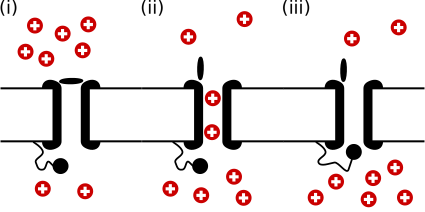
\includegraphics{figures/intro/activation_gate}
\end{center}
\caption[Time-Dependent Ion Channel]{
\label{fig:intro:heart:gated_ion}
A time dependant ion channel, represented by the black structure which bisects
the membrane (horizontal lines) for positive ions, shown as red circles.
The channel has an activation gate, the black lozenge on the top of the
membrane and an inactivation gate, the ball and chain on the underside of the
membrane.
In panel (i) the gate is not activated and shows a large concentration of ions
on the upper side.
In panel (ii), the gate activates and ions flow down the channel to the region
of lower concentration.
In panel (iii), the inactivation gate has moved to close the channel and no more
ions flow.
}
\end{figure}


Many gated channels are what are known as time-dependent channels.
These channels have structures over one or both ends which modulate the total
conductance to open (activate) or close (inactivate) the channel.
This is illustrated in figure~\ref{fig:intro:heart:gated_ion}.
The time course of this activation or inactivation is normally modulated by the
voltage, but can also be modulated by ion concentration or other mechanisms.

\begin{figure}
\begin{center}
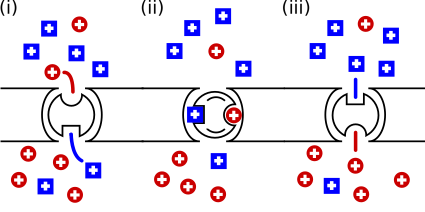
\includegraphics{figures/intro/ion_pump}
\end{center}
\caption[Ion Pump]{
\label{fig:intro:heart:ion_pump}
An ion pump (or more accurately, an ion exchanger), represented by the black
structure which bisects the membrane (horizontal lines) for two species of
positive ion, represented by red circles and blue squares.
The pump works against the concentration gradient.
In panel (i), the two ions bind to their respective sites on the pump.
In panel (ii), the pump changes its structure, drawing each ion through the
membrane.
In panel (iii), the pump releases the binding of the ions, letting them rejoin
the free ion populations.
}
\end{figure}

Pumps use energy to actively move ions against the gradient.
Complex molecules latch onto the ions on one side of the membrane and move them
through to the other side.
Many pumps are actually exchangers, which take in ions of one sort on one side
whilst transporting another type of ion the other way.

\subsubsection{Myocyte Electrical Action Potentials}

The evolution of the electrical state of the cell, from polarised to depolarised
and back again is termed the action potential (AP).
The shape and duration of
the action potential is mostly determined by the channels, carriers and pumps
across the cellular membrane, though the internal and external concentrations of
several ions and molecules can also have a significant effect.
There are three
principle ion species involved in the development of the action potential;
sodium ($\text{Na}^{\text{+}}$), potassium ($\text{K}^{\text{+}}$) and calcium
($\text{Ca}^{\text{2+}}$).
The third, calcium, is also important for contractile function.
Chlorine ($\text{Cl}^{\text{-}}$) is also of importance in some cells.

\begin{figure}
\begin{center}
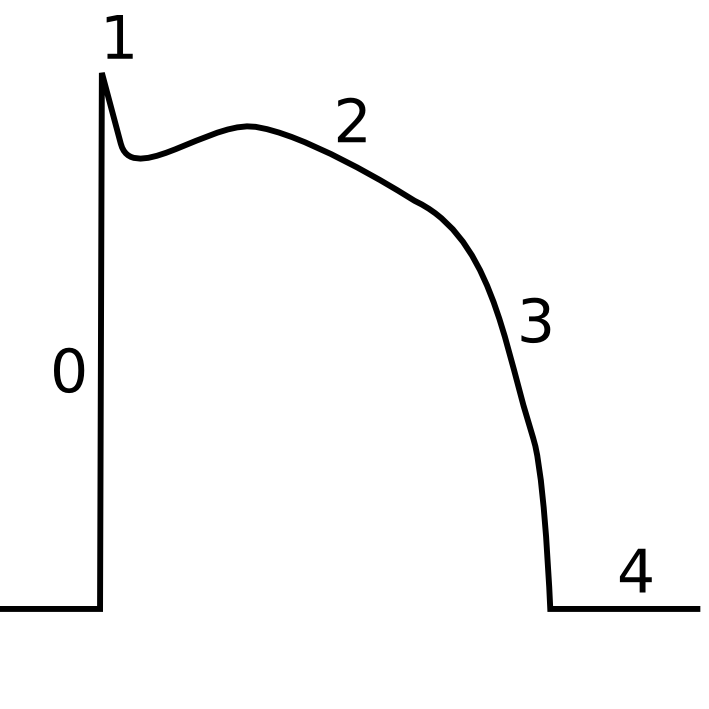
\includegraphics{figures/intro/ap_profile}
\end{center}
\caption[Schematic AP Profile]{
\label{fig:intro:heart:ap}
A schematic AP profile.
Labelled are the five phases of the action potential.
Phase 0, the upstroke.
Phase 1, the end of the upstroke.
Phase 2, the plateau.
Phase 3, the repolarization.
Phase 4, the resting period.
}
\end{figure}

The action potential has 5 phases (figure~\ref{fig:intro:heart:ap}).
It begins with depolarization, phase 0.
During depolarisation, the current is carried principally by the fast inward
sodium current.
Phase 0 is also known as the upstroke of the action potential, and its slope is
important to the propagation of the action potential through cardiac tissue and
also the excitability of the myocyte as in individual cell.
Phase 0 is over almost instantaneously in healthy myocytes.

Phase 1 signifies the end of the upstroke, and is caused by the inactivation of
the sodium channels.
The small notch present in some cellular action potentials is caused by a
transient net outward current, carried principally by potassium.

Phase 2 is the plateau phase.  This relatively long phase ($>$100ms in some
myocytes) is due to the balance of slowly activating inward calcium currents and
the outward potassium currents.
The inward calcium current is principally carried by the L-type calcium channels
and the outward potassium current by a plethora of channels, classified by the
speed of activation or the substance which modulates them.

Phase 3 is the repolarization period.
The calcium channels have inactivated.
The potassium currents are still open, and the net efflux of positive charge
repolarizes the cell.

The final phase 4 is the period during which the cell is at the resting
potential.
In addition, for a short period of phase 4, the cell is in fact
impossible to excite above this resting potential due to the inactivations of
numerous channels.
This is called the refractory period.

Both the shape and the length of the action potential have physiological
importance.
Many pathological conditions have a significant impact upon both.
The action potential duration (APD) is often given as an \apd\ or
\apd[50], denoting the duration of the AP at 90\% or 50\% repolarization,
respectively.

\section{Mathematical Models of the Heart}

Cardiac tissue has been modelled mathematically for about fifty years.
While initial models were simple, there are now models of high sophistication
available.
These models are capable of reproducing both healthy and pathological behaviour
with some accuracy.

\subsection{Categorising Myocyte Models}

Cellular models tend to be classified in two ways.
The first differentiator is the level of detail employed.
The second is on which cellular processes are modelled.

Biophysically detailed models are complex.
They consider the interactions of several different currents, and potentially
intra- and extracellular ion concentrations, reservoirs as well as other
details.
The second type are simplified, phenomenological, models.
These do not consider individual ion concentrations but instead just reproduce
one desired factor, typically the action potential profile.

Models, whether biophysically detailed or not, can concern themselves with the
cellular electrophysiology, the mechanical contrations or both.
This thesis concerns itself just with electrophysiological models.
Models of the mechanics are not considered and are not treated in this
description of mathematical modelling.

\subsection{A Brief History Of Cardiac Myocyte Modeling}

The first model of cardiac electrophysiology was published by
Noble~\cite{Noble1962}, and modelled Purkinje fibre (A specialised part of the
ventricular conduction system) action potentials.
Shortly thereafter, various refinements were published, as further experimental
data became available.
This was eventually followed by the Beeler--Reuter~\cite{Beeler1977}\ model of
the guinea pig ventricular myocyte.

The Luo--Rudy guinea pig ventricular myocyte model was first published in
1991~\cite{Luo1991} and was then sub-sequentially majorly revised and
republished in 1994~\cite{Luo1994}.
The first Luo-Rudy model was based on the Beeler--Reuter model, though with updated channel behaviours
and more complex potassium channels.
The second Luo-Rudy model was the first of the `second generation' models,
with fluctuations in all ion concentrations, and a much more detailed series of
equations for calcium handling.

In 1998, the Courtemanche--Ramirez--Natel\cite{CRN98}\ (CRN) model and the
Nygren~\cite{Nygren1998}\ model were published.
These were both models of the human atrium.
They were also both second generation models, with detailed calcium handling.
Also in 1998 Fenton and Karma published their phenomenological
Fenton--Karma~\cite{Fenton1998}\ model, which used just three channels to
reproduce the shape of the ventricular action potential.

\subsection{Mathematical Models of Myocytes}

Mathematical models of cardiac myocytes are built from a few simple assumptions
and considerations.
These concern the behaviour of the cellular membrane and ion channels.
The important ones are detailed here.

\subsubsection{Electric Circuit Model}

The electrical circuit model of the cell membrane underpins much of the work in
modelling the behaviour of cardiac myocytes.
It is however a very simple concept.
Since the membrane seperates charges, it may be considered as a capacitor, as
shown in figure~\ref{fig:intro:math:circuit}.
Since there is no net buildup of
charge on either side of the membrane, any ionic current, \ii{ion}, must be
countered by a capacitive current, and so
\begin{equation}
C_{m}\frac{dV_{m}}{dt} + \ii{ion} = 0
\label{eqn:intro:math:basic}
\end{equation}
where $V_{m}$ is the membrane voltage, and is defined as the difference between
the internal potential, $u_{i}$ and the external potential, $u_{e}$ or
\begin{equation}
V_{m} = u_{i} - u_{e}
\label{eqn:intro:math:vm}
\end{equation}
When multiple currents are considered, the total inward and outward currents are
summed.
The difficulty comes in determining the form of \ii{ion}, which varies widely
depending on the nature of the channel or pump in question.

\subsubsection{The Nernst Equilibrium Potential}

The Nernst equation is an important equation in electrophysiology.
It describes how the difference in ion concentrations on two sides of a
semi-permeable barrier can result in a potential difference across the barrier.
Any voltage dependant factor of a current of an ion, S, includes a reversal
potential, V$_{S}$, equal to the Nernst potential.
At the reversal potential, the current falls to 0.
When equilibrium is reached the potential difference, $V_{S}$, across the
membrane is given by
\begin{equation}
V_{S} = \frac{RT}{zF}ln\left( \frac{[S]_{e}}{[S]_{i}} \right) 
\end{equation} 
where subscripts $i$ and $e$ denote internal and external concentrations of S,
$R$ is the universal gas constant, $T$ is the absolute temperature, $F$ is
Faraday's constant and $z$ the charge of the ion $S$.

The Nerst Potential applies only to a single ion concentration.
This is not as large a limitation as it first might seem.
Whilst the action potential involves many ion species, many channels are ion
specific and thus the Nerst potential applies across them.

\subsubsection{The Hodgkin-Huxley Equations}

Many mathematical models of cardiac myocytes feature one or more
`Hodgkin--Huxley' channels.
Hodgkin and Huxley developed them in a now classic series of papers concerning
the current flow through the membrane of the squid giant axon.
They characterise the current flow with elegance and surprising accuracy.
It is important to note that the Hodgkin--Huxley equations consider the bulk
behaviour of the many thousands of individual channel structures distributed
across the membrane, not the behaviour of one single channel.

Hodgkin and Huxley started with a very simple assumption.
The current flow through a channel on the membrane, $I_{S}$ is given by
\begin{equation}
I_{S} = g_{S}\left(V-V_{S}\right)
\label{eqn:intro:math:hh1}
\end{equation}
where $g_{S}$ is the channel conductance, $V$ the membrane potential and $V_{S}$
the Nernst potential for the ion S.
Equation (\ref{eqn:intro:math:hh1}) assumes that the channel is selective for
one ion species S, and that the current is a simple linear function of the
voltage across the membrane.

With this underlying assumption, Hodgkin and Huxley set out to accurately map
the behaviour of the current with regards time and voltage.
The following section explains the description for the sodium current, \ii{Na}.
From the form of the sodium channel under voltage clamp conditions, it is
reasonable to expect $g_{Na}$ obeys a differential equation of the form
\begin{equation}
\frac{dg_{Na}}{dt} = f\left(v,t\right)
\label{eqn:intro:math:hh2}
\end{equation}
where $v=V-V_{Na}$.
However, the form of $g_{Na}$ is complex.
While remaining at the same voltage, the conductance at first increases and then
tails off.
It appeared that there were two processes at work, one that turned the current
on, and one that turned it off.
Hodgkin and Huxley realised that it would be easier to write $g_{Na}$ as a
function of two different variables.
One which corresponded to the turning on and one to the turning off of the
channel.
This leads there being an activation variable, called $m$, an inactivation
variable, called $h$ and that the current would be some linear combination of the
two, multiplied by a constant conductance factor $\bar{g}_{Na}$.
The two variables $m$ and $h$ would both satisfy a differential equation such as
\begin{equation}
\frac{dm}{dt}=\alpha_{m}\left(v\right)\left(1-m\right) -
\beta_{m}\left(v\right)m
\label{eqn:intro:math:dmdt}
\end{equation}
where $\alpha_{m}$ and $\beta_{m}$ are functions of $v\,\left(=V-V_{Na}\right)$.
As an activation $m$, $\alpha_{m}$ and $\beta_{m}$ are such that $m$ is
initially small but increases with the potential.
As $h$ is an inactivation, $\alpha_{h}$ and $\beta_{h}$ give an initially high
value of $h$ that then decays, inactivating the channel.

The form proposed for $g_{Na}$ by Hodgkin and Huxley was
\begin{equation}
g_{Na}=\bar{g}_{Na}m^{3}h
\label{eqn:intro:math:gna}
\end{equation}
where all symbols are as defined previously.
The decision to raise $m$ to the third power was based on the rate of increase
observed in voltage clamp experiments.
It is interesting to note that when the structure of \ii{Na}\ was examined in
detail, it was discovered that the channel has three structures which open to
allow current to flow.
A second structure, the `ball and chain' then acts to close the channel.

Many different channels are modelled as Hodgkin--Huxley channels.
Different channels have different activation and inactivation variables.
These variables are modulated by different $\alpha$ and $\beta$ equations.

\subsubsection{Markov Chain Channels}

Markov chain models of ion channels~\cite{Balser1990,Clancy1999,Silva2005}\
emerged when more detailed information on ion channel behaviour became
available.
This included single channel recordings rather than whole cell recordings.
Under such conditions, as well as in certain pathological states, the
Hodgkin--Huxley descriptions of the cells broke down.

In a markov chain model, instead of having one or more activations or
inactivations, the channel has a number of states.
Common states can include open, inactive and closed.
A channel can have more than one state of each sort.
Transitions are only allowed between certain states and each transition has a,
usually time or voltage dependent, probability.
Channels only allow current to flow whilst in an open state.

Markov chain models can be highly complex and contain many states.
They can be utilised in a variaty of ways.
One markov chain can represent the behaviour of all the individual channels on
the cell.
In this case, the total current flowing in the channel will be proportional to
the fraction of open states.
Cells can also have multiple markov chains to represent the flow through a
channel, each with its own proportions of state occupancy.
They also open the possibility of using stochastic simulation techniques where
the transition between states is controlled by random chance.

\subsection{Selected Myocyte Models}

There are tens, perhaps hundreds, of myocyte models of varying complexity and
accuracy.
There are relatively few models of atrial myocytes for human tissue.
A brief description of the foremost two are given here, as well as a description
of one of the most adaptable phenomological models.

\subsubsection{The Courtemanche--Rameriz--Nattel Model}

The Courtemanche--Rameriz--Nattel (CRN) model~\cite{CRN98}\ is a biophysically
detailed second generation model of the human atrial myocyte.
It was based on the Luo-Rudy~\cite{Luo1994}\ model of the guinea pig ventricular
myocyte.
The currents were then modified based on data from human and animal atrial
myocytes.

The CRN model tracks 21 state variables.
Most of these are gating parameters for the many ion channels, but the model
also tracks the internal concentration of potassium, sodium and calcium ions.
The external concentrations of ions are assumed constant.
There are also state parameters representing the calcium stored in internal
structures, such as the sarcoplasmic reticulum.
\begin{equation}
\label{eqn:intro:math:crn}
\ii{ion} = \ii{Na} + \ii{K1} + \ii{to} + \ii{Kur} + \ii{Kr} + \ii{Ks} +
\ii{Ca,L} + \ii{b,Na} + \ii{b,Ca} + \ii{NaK} + \ii{NaCa} + \ii{p,Ca}
\end{equation}
The CRN has 12 transmembrane currents which contribute to \ii{ion},
equation~(\ref{eqn:intro:math:crn}), and pumps and 4 currents and
pumps which just interact with the internal calcium stores.
The external currents are \ii{Na}, the fast sodium current, \ii{K1}, the inward
rectifier calcium current, \ii{to}, the transient outward current, \ii{Kur}, the
ultra-rapid delayed rectifier current, \ii{Kr}, the rapid delayed rectifier
current, \ii{Ks}, the slow delayed rectifier current, \ii{Ca,L}, the L-type
calcium current, \ii{b,Na}, the sodium background current and \ii{b,Ca}, the
calcium background current.
All the currents are time-dependent, except for the background currents which
have constant coductance and \ii{K1}, which is voltage-dependent.
There are also three pumps; \ii{NaK}, the sodium--potassium exchanger,
\ii{NaCa}, the sodium--calcium exchanger and \ii{p,Ca}, the calcium pump.

As a biophysically detailed model, the CRN model is suitable for a variety of
modeling tasks.
The number of currents make it an attractive option for modeling drugs or
genetic mutations.
It can be expensive to solve for large numbers of cells, however.

\subsubsection{The Nygren Model}

The Nygren model~\cite{Nygren1998}\ is a biophysically detailed second
generation model of the human atrial myocyte.
It was based on the Linblad~\cite{Lindblad1996} model of the rabbit atrium.
The equations were then modified using human data, mostly gathered from the
atrial appendages.

The Nygren model tracks 29 state variables.
Most of these are gating parameters.
They model also tracks concentrations of ions, both internally and in
extracellular cleft spaces, to represent local ion fluctuations.
Like the CRN model, there are also variables to represent internal calcium
handling.
\begin{equation}
\label{eqn:intro:math:nygren}
\ii{ion} = \ii{Na} + \ii{K1} + \ii{to} + \ii{Kur} + \ii{Kr} + \ii{Ks} +
\ii{Ca,L} + \ii{b,Na} + \ii{b,Ca} + \ii{NaK} + \ii{NaCa} + \ii{p,Ca}
\end{equation}
The Nygren model has 12 transmembrane currents which contribute to \ii{ion},
equation~(\ref{eqn:intro:math:nygren}), and pumps and 4 currents and
pumps which just interact with the internal calcium stores.
The external currents are \ii{Na}, the fast sodium current, \ii{K1}, the inward
rectifier calcium current, \ii{to}, the transient outward current, \ii{Kur}, the
ultra-rapid delayed rectifier current, \ii{Kr}, the rapid delayed rectifier
current, \ii{Ks}, the slow delayed rectifier current, \ii{Ca,L}, the L-type
calcium current, \ii{b,Na}, the sodium background current and \ii{b,Ca}, the
calcium background current.
All the currents are time-dependent, except for the background currents which
have constant coductance and \ii{K1}, which is voltage-dependent.
There are also three pumps; \ii{NaK}, the sodium--potassium exchanger,
\ii{NaCa}, the sodium--calcium exchanger and \ii{p,Ca}, the calcium pump.

The Nygren model is a biophysically detailed model, suitable for a variety of
modelling tasks.
It has more involved mathematics and requires more storage than the CRN model,
making it less attractive for large-scale simulation.
It is also interesting to note that the two models have very different
AP morphologies, the reasons for which have been the subject of some
research~\cite{Nygren2001,Syed2005,Cherry2008}.

\subsubsection{The Fenton--Karma Model}

The Fenton--Karma (FK) model~\cite{Fenton1998,Bueno-Orovio2008}\ is a
phenomenological, or minimal variable, model of the ventricular action
potential.
The goal of the FK model is to accurately reproduce the AP profile and
restitution properties of myocytes as well as short-term memory effects.
The original FK model has 3 variables, a fourth was added recently.

The FK model tracks 4 state variables.
These have no real physiological analogues.
\begin{equation}
\label{eqn:intro:math:fko}
\ii{ion} = \ii{fi} + \ii{si} + \ii{so}
\end{equation}
The FK model has 3 transmembrane currents which contribute to \ii{ion},
equation~(\ref{eqn:intro:math:fko}).
The fast inward current, \ii{fi}, is roughly analogous to the fast sodium
current in more detailed models, the slow inward current, \ii{si}, fulfils a
similar role to the L-type calcium current and the slow outward current, \ii{si},
is analogous to the potassium rectifier currents.
The behaviour of the currents is generally controlled by step functions based
on the state variables.

The FK model is not biophysically detailed.
This makes it very fast to solve, making it attractive for large tissue
simulations.
The drawback of this is that incorporating complex hormonal or drug interactions
is difficult.
The model is highly modifiable, with parameter sets that can reproduce a variety
of AP morphologies and restitution behaviours, including one for atrial myocyte
APs~\cite{Weber2008}.

\subsection{Action Potential Propagation}

Single myocyte models are important, and can tell us much about the heart in
disease and health.
The heart is not made up of isolated myocytes however.
Whilst current computational power does not allow myocytes to be modelled on an
individual cellular basis for the whole heart, continuum models of propagation
have been developed.
These are summed up in the bidomain equations, and their simplification, the
monodomain equations.

\subsubsection{The Bidomain Equation}

The bidomain equation comes out of basic electromagnetic theory and several
assumptions about the nature of cardiac tissue~\cite{Tung1978,Geselowitz1983}.
\begin{enumerate}
    \item The cardiac tissue contains two continuous, simply connected domains, the intracellular and extracellular domains.
    There is no detailed consideration of the fine points of geometry.
    \item The intra- and extracellular domains overlap and fill all of the cardiac muscle. Each point lies in both domains.
    \item Charge does not accumulate.
\end{enumerate}

The derivation is not that difficult to work through, and it results in the bidomain equations
\begin{align}
\underline{\nabla}\cdot\left(\left(M_{i}+M_{e})\right)\underline{\nabla}u_{e}\right) + \underline{\nabla}\cdot\left( M_{i}\underline{\nabla}V_{m}\right) &=& 0
\label{eqn:intro:math:bidom1}\\
\underline{\nabla}\cdot\left(M_{i}\underline{\nabla}V_{m}\right) + \underline{\nabla}\cdot\left(M_{i}\underline{\nabla}u_{e}\right) &=& \chi C_{m}\frac{dV_{m}}{dt} + \chi{I_{ion}}
\label{eqn:intro:math:bidom2}
\end{align}
where the subscript $i$ and $e$ refer to the intra- and extracellular quantities, $M$ is a matrix of conductivities, $\chi$ represents the surface-to-volume ratio of the cells and all other quantities are as defined previously.
The bidomain equations are a coupled set of a parabolic and elliptic differential equation.

Boundary conditions for the bidomain equations vary, though the most common ones are described here.
First, no intracellular fluxes leave the heart.
Second, the body is assumed to be a passive conductor that is isolated at the outer surface.
The body potential at the surface of the heart is the extra-cellular potential at the surface of the heart.

\subsubsection{The Monodomain Equation}

While the bidomain equations represent a good tool for modelling some of the complexities of cardiac conduction, they are very demanding to solve, necessitating finding the solution to coupled parabolic and elliptic differential equation sets.
The monodomain equation is the result of one simplifying assumption made to the bidomain equations.
For the monodomain equation, we assume that the anisotropy ratio, $\lambda$, is the same for the intra- and extra-cellular fluids at all points.
\begin{equation}
M_{i} = {\lambda}M_{e}
\label{eqn:intro:math:mratio}
\end{equation}
This assumption is not a very physiological one, but the simplification it
allows is significant and so it is quite commonly used.

Substituting (\ref{eqn:intro:math:mratio}) into (\ref{eqn:intro:math:bidom1})
and (\ref{eqn:intro:math:bidom2}) and rearranging reduces the pair of equations
to one single equation for the membrane potential
\begin{equation}
\frac{\lambda}{1+\lambda}\underline{\nabla}\cdot\left(M_{i}\underline{\nabla}V_{m}\right) = \chi C_{m}\frac{dV_{m}}{dt} + \chi{I_{ion}}
\label{eqn:intro:math:mono}
\end{equation}
Typically, the factor of ${\lambda}/\left({1+\lambda}\right)$ is folded into $M_{i}$ to give the diffusion tensor $D$.
In 1D, this is the cable equation, which is very widely used.
The values of the components of the tensors $M_{i}$ or $D$ may be determined experimentally, or from a comparison of conduction in real and virtual tissue samples.

\subsection{Solving Mathematical Models}

There exist a wealth of techniques for solving the ordinary differential
equations (ODEs) and partial differential equations (PDEs) involved in
mathematical models.
These techniques vary in complexity and accuracy.
The correct choice of technique depends on a number of factors including the
`stiffness' of the equations, the desired accuracy and others.

\subsubsection{Forward Euler Method}

\subsubsection{The Finite Difference Method}

\subsubsection{The Rush--Larsen Technique}

\section{The Electrocardiograph}

The electrocardiograph, or ECG, was developed by Einthoven and colleagues at the
turn of the 20th century.
The Einthoven ECG used the string galvanometer, developed by Einthoven, to
record the potential differences between three sets of electrodes, or leads.
These electrodes were placed on each arm and on the left leg.
These three electrodes form the bases of many ECGs recorded to this day.
The string galvanometer was highly sensitive electrical recording device for its
time, and was developed by Einthoven.
For the development of the ECG and the string galvanometer, Einthoven was awarded
the nobel prize in 1924~\cite{Kligfield2002,Levick1991}.

Since Einthoven's day, the ECG has been continually refined.
This refinement has included both improvements in the way that individual leads
are measured, and new leads that are recorded.
In addition, there have been a number of specialised lead sets developed for
particular purposes, such as exercise recording and 24 hour measurement.
Research into new lead sets, to better understand the functioning of the heart,
continues to this
day~\cite{Jahrsdoerfer2005,Sobieszczanska2007,Grube2007,Finlay2007}.

\subsection{Lead Theory}
\label{sec:intro:ecg:lead_theory}

In Einthoven's original conception of the heart and the electrical field it
produced, he developed the `Einthoven Triangle'.
The Einthoven triangle is an equilateral triangle.
At its corners sit the three electrodes and the sides of the triangles are the
leads themselves.
At the centroid of the triangle sits the heart, which is represented by a
single, stationary, time varying dipole.
The potentials measured at the three electrodes are the potentials assuming the
system is two dimensional, homogeneous and infinite in extent.
This is not entirely incorrect.

Modern lead theory was developed in the 1950's.
In a series of three papers McFee and
Johnston~\cite{McFee1953,McFee1954a,McFee1954b}\ set out their concept of the
`lead field' which is still considered applicable today.
This theory, which was a further generalisation of work by Burger and van
Milaan, allows for a heart which consisted of distributed dipole sources
sitting in a three dimensional, finite and inhomogeneous medium.

First, it is useful to define what a lead is.
A lead is defined as a pair of terminals, each connected to any number of electrodes
on the body, either directly or through any number of resistors or amplifiers.
One of the terminals is designated (arbitrarily) as the `positive' terminal.
The terminals are connected such that a positive measurement is taken if
the `positive' terminal has a higher potential than the `negative' one.

The lead field theory is based on the fundamental principles of linear volume
conductors set out by Helmholtz in the middle of the nineteenth century.
These principles only hold if the body can be treated as a linear volume
conductor.
This is a good approximation~\cite{Geddes1967}.

The first principle, that of superposition, states that the electric field
resulting from several sources in the medium is equal to the sum of the fields
which would be produced by each source considered alone.
The second principle, that of reciprocity, concerns current flow in the
medium.
It states that the current flow between two electrodes evoked by a field source in the
medium is the same as the current flow through the source evoked by placing a
potential difference across the two electrodes equal to the potential difference
that would have been created by the field source.
That is to say that the current flow is independent of the direction of
energisation, from within or outside the medium.

\begin{figure}
\begin{center}
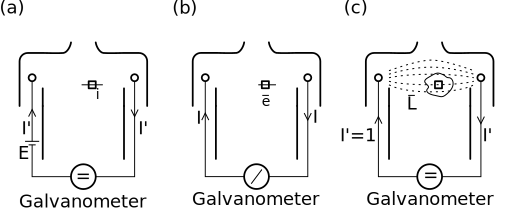
\includegraphics{figures/intro/lead_field}
\end{center}
\caption[Diagram of the Reciprocity Principle and the Lead Field]{
\label{fig:intro:ecg:lead_field}
Diagram of the Reciprocity Principle and the Lead Field.
(a) Inducing a current in the lead $l$, between the terminals of the
galvanometer causes an electric field which causes a current $i$ to flow through
the small element (square) in the heart.
(b) An electric field, $\vec{e}$, generated by the small element causes a current
I to flow in $l$ causing the galvanometer to read the potential difference $E'$.
If $E'$ equals $E$ then $I$ equals $i$.
(c) The lead field, $\vec{L}$, is defined from the current which flows in each
small unit of the heart when the current introduced is the unit current.

}
\end{figure}

To derive the lead field, we consider a unit current flowing in a
lead $l$~(figure~\ref{fig:intro:ecg:lead_field}).
The resulting flow of current through the body will have a certain magnitude and
direction at every point; it is a vector field.
This vector field is called $\vec{L}$, the lead field.
If one considers a small volume in the heart region of the torso then the
presence of the lead field, $\vec{L}$, will set up an electric field in the
volume, $\vec{e}$.
The principle of reciprocity means that if instead the electrical activity of
the heart creates an electric field, $\vec{e}$, in the heart region then a unit
current will flow through the lead $l$.
The principle of superposition allows the contributions of many such small
volumes, each containing their own field, $\vec{e_1},\cdots,\vec{e_n}$, to
create a current, and thus a potential difference in $l$.


\subsection{The Twelve Lead Electrocardiogram}

The twelve lead electrocardiograph is the initial basis of almost all cardiac
diagnosis.
It started out as the three einthoven leads.
The electrodes are located (figure~\ref{fig:intro:ecg:leads})(a)) on the left
shoulder, L, the right shoulder, R, and the feet (typically the left leg), F.
Lead I (\ref{eqn:intro:leads:i}) uses R as the negative terminal and L as the
positive terminal.
Lead II (\ref{eqn:intro:leads:ii}) is formed between R as the negative terminal
and F as the positive terminal.
Lead III (\ref{eqn:intro:leads:iii}) is formed between L as the negative terminal
and F as the positive terminal.

\begin{figure}
\begin{center}
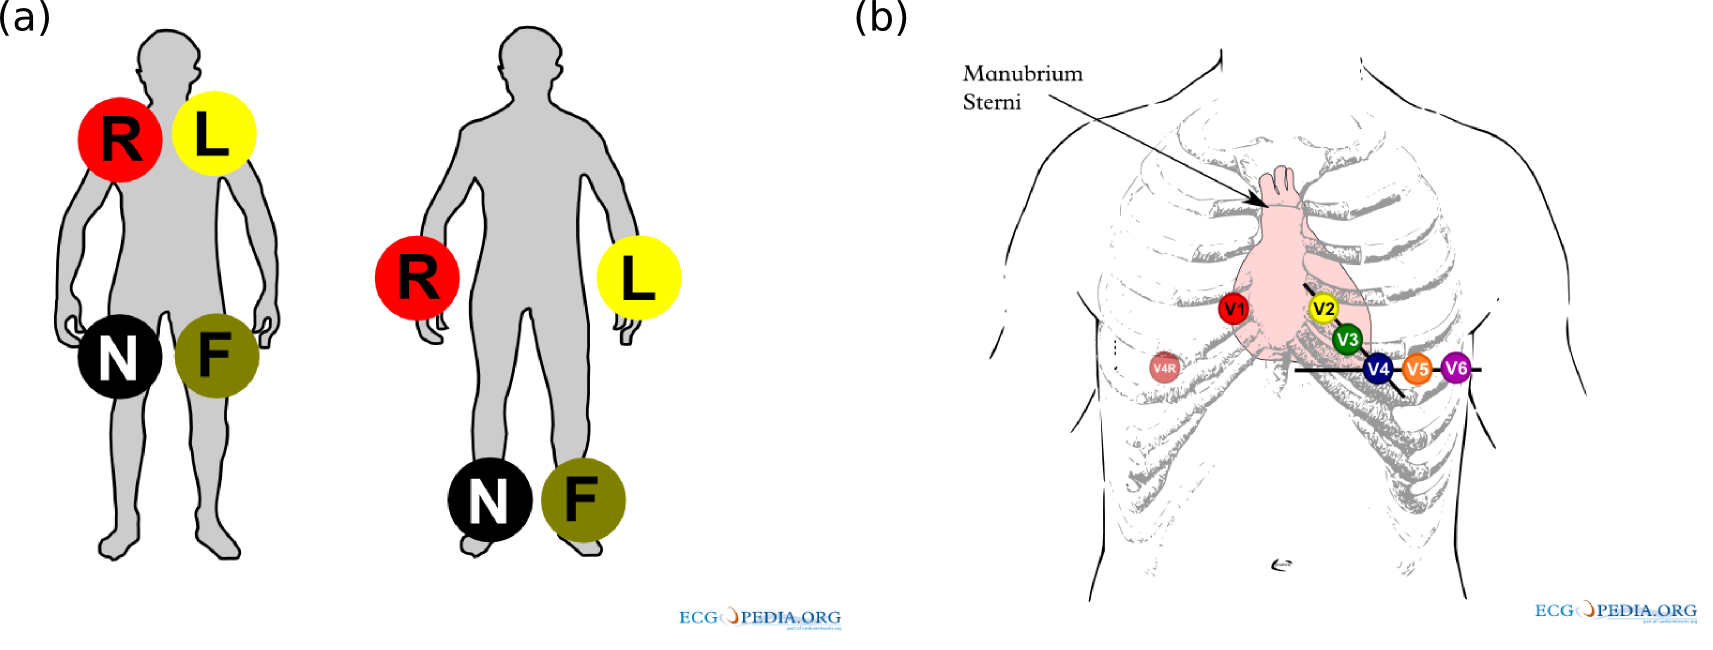
\includegraphics{figures/intro/ecg_leads}
\end{center}
\caption[Lead placements for the 12 Lead ECG]{
\label{fig:intro:ecg:leads}
Lead placements for the 12 lead ECG.
(a) Placement of the three limb leads, L, R and F, as well as the ground
electrode N.
(b) Placement of the six precordial electrodes, $\text{V}_{\text{1--6}}$.

Images are reproduced from the ECGpedia~\cite{ecgpedia}.
Both are kindly released under a Creative Commons
Attribution-Noncommercial-Share Alike 3.0 Netherlands License.
}
\end{figure}

Wilson~\cite{Wilson1934}, in the 1930s, introduced an indifferent
electrode,  constructed by averaging the potentials at the three limb
electrodes (\ref{eqn:intro:leads:wct}).
This is the Wilson's central terminal (WCT).
They introduced three new `unipolar' leads, all of which use the WCT as the
negative terminal.
For the positive terminal, VL uses the L electrode, VR the R electrode and VF
the F electrode.
Later Goldberger~\cite{Goldberger1942}\ noted that be removing the electrode used
as the positive terminal from the calculation of the central terminal for the
negative electrode, the amplitude of the lead would be 50 per cent larger than
that of the normal unipolar leads.
These leads were termed the augmented unipolar leads, denoted by the prefix of
an `a'.
The aVL (\ref{eqn:intro:leads:avl}) leads uses L for the positive terminal and
the average of R and F for the negative terminal.
The aVR (\ref{eqn:intro:leads:avr}) leads uses R for the positive terminal and
the average of L and F for the negative terminal.
The aVF (\ref{eqn:intro:leads:avf}) leads uses F for the positive terminal and
the average of R and L for the negative terminal.
The set of leads consisting of I, II, III, aVL, aVR and aVF are known as the
limb leads.
The superior limb leads are I, aVL, aVR and the inferior are II, III, aVF.

The precordial leads were introduced by Wilson~\cite{Wilson1944}\ to provide a
better view of the electrical activity of the heart from the chest.
They are all unipolar leads which use the WCT for the negative
terminal.
For the positive terminal they use one of the six precordial electrodes
(figure~\ref{fig:intro:ecg:leads})(b), the locations of which are described in
many textbooks (e.g.  \cite{Hampton2008}).
The first precordial electrode, which is the positive terminal of
$\text{V}_{\text{1}}$ (\ref{eqn:intro:leads:v1}) is located to the right of the
sternum, in the fourth intercostal--between the ribs--space.
The second precordial electrode, which is the positive terminal of
$\text{V}_{\text{2}}$ (\ref{eqn:intro:leads:v2}) is located to the left of the
sternum, in the fourth intercostal space.
The third, the positive terminal of $\text{V}_{\text{3}}$
(\ref{eqn:intro:leads:v3}) is located between the second and fourth precordial
electrodes.
The fourth ($\text{V}_{\text{4}}$, \ref{eqn:intro:leads:v4}) is located on the
left midclavicular line, in the fifth intercostal space.
The fifth ($\text{V}_{\text{5}}$, \ref{eqn:intro:leads:v5}) is located on the
left anterior axillary line, in the fifth intercostal space.
The sixth ($\text{V}_{\text{6}}$, \ref{eqn:intro:leads:v6}) is located on the
left positerior axillary line, in the fifth intercostal space.

The voltage, $V$, across each lead can be written as
\begin{subequations} \label{eqn:intro:leads}
\begin{align}
V_{I}  = &\phi_{L} - \phi_{R}\label{eqn:intro:leads:i}\\
V_{II}  = &\phi_{R} - \phi_{F}\label{eqn:intro:leads:ii} \\
V_{III}  = &\phi_{L} - \phi_{F}\label{eqn:intro:leads:iii}\\
V_{WCT}  = &\frac{\phi_{L} + \phi_{R} + \phi_{F}}{3}\label{eqn:intro:leads:wct}\\
V_{aVL} = &\phi_{L} - \left(\frac{\phi_{R} + \phi_{F}}{2}\right) \label{eqn:intro:leads:avl}\\
V_{aVR} = &\phi_{R} - \left(\frac{\phi_{L} + \phi_{F}}{2}\right)\label{eqn:intro:leads:avr} \\
V_{aVF} = & \phi_{F} - \left(\frac{\phi_{R} + \phi_{L}}{2}\right)\label{eqn:intro:leads:avf}\\
V_{1} = & \phi_1 - V_{WCT} \label{eqn:intro:leads:v1}\\
V_{2} = & \phi_2 - V_{WCT} \label{eqn:intro:leads:v2}\\
V_{3} = & \phi_3 - V_{WCT} \label{eqn:intro:leads:v3}\\
V_{4} = & \phi_4 - V_{WCT} \label{eqn:intro:leads:v4}\\
V_{5} = & \phi_5 - V_{WCT} \label{eqn:intro:leads:v5}\\
V_{6} = & \phi_6 - V_{WCT} \label{eqn:intro:leads:v6}
\end{align}
\end{subequations}
where $\phi_x$ is the potential measured at electrode $x$.

As there are only 9 electrodes in the twelve lead ECG, there are only 8
potential differences which can be uniquely determined.
These are, by convention, leads I, II and $\text{V}_{\text{1--6}}$.
The value of the other limb leads is that they provide a view of the activity of
the heart from different angles, thus what might be unclear on one lead can be
obvious on another.
This concept of lead angles creates what is known as the hexaxial reference
system (\cite{Lipman1994}, pp 94., amongst others), illustrated in
figure~\ref{fig:intro:ecg:hex}.
The angle at which each lead points is the direction of the positive terminal.
Lead I, which is nominally horizontal, is at \degr{+0}.
Under the hexaxial system, Lead II has an angle of \degr{+60}\ and lead III,
\degr{+120}.
The unipolar limb leads (both augmented and not) have angles of \degr{-30}\ for
aVL, \degr{+90}\ for aVF and \degr{-150}\ for aVR.

\begin{figure}
\begin{center}
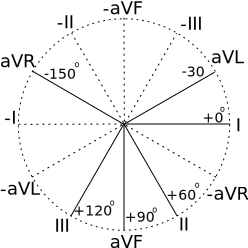
\includegraphics{figures/intro/hexaxial}
\end{center}
\caption[Hexaxial Reference System]{
\label{fig:intro:ecg:hex}
Diagram of the hexaxial reference reference system, showing the nominal
directions of the 6 limb leads.
The positive senses of the leads are in bold, the negative are dashed.
\degr{+0}\ is horizontal and to the left, in the reference frame of the body.
}
\end{figure}

\subsection{The ECG Waves}

\begin{figure}
\begin{center}
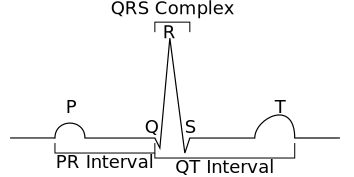
\includegraphics{figures/intro/schematic_ecg}
\end{center}
\caption[Schematic ECG]{
\label{fig:intro:ecg:schematic}
A schematic representation of the ECG in lead II.
Shown are the P-wave, the QRS complex and the T-wave.
Also indicated are two important time periods; the PR interval and the QT
interval.
}
\end{figure}

In terms of the ECG, a `wave' is a deflection from the baseline observed in the
lead.
There are five standard waves in the ECG; P, Q, R, S and T.
The origin of the names of these waves is a matter of some
controversy~\cite{Hurst1998}, but whatever their origin, they are now enshrined
in the literature.
A schematic representation of the ECG waves is shown in
figure~\ref{fig:intro:ecg:schematic}.
Each of the waves is the result of the electrical activity in a particular part
of the heart.
Positive deflections are those which are above the baseline and negative ones
below.

The P-wave is caused by the depolarisation of the atria.
It has a relatively low amplitude because the atria are small and thin walled
compared to the ventricles, so there are not that many cells which can generate
the wave.
It tends to last from \ms{100} to \ms{120}.

The QRS complex is associated with the ventricular depolarisation.
It is a collection of up to three waves.
Any negative deflection which preceeds the R wave is the Q wave.
The R wave is the first positive deflection.
The S wave is the first negative deflection after the R wave.
A QRS complex does not need to have all three of the QRS waves present.
The QRS complex tends to have the largest magnitude in the ECG and lasts
approximately \ms{100}.

The T wave is associated with the ventricular repolarization.
It occurs some time after the QRS complex.
The $\text{T}_{\text{P}}$, caused by the atrial repolarization is not normally
visible on the ECG for a number of reasons.
It is very small in magnitude, it is also often masked either by the QRS complex
or by so called `baseline correction' algorithms which use the PR interval to
determine a `zero' for the ECG.

The axis of a wave is direction in which it has maximum amplitude.
This is determined using the hexaxial reference system.
A normal QRS complex (\cite{Lipman1994,Katz2006}) has an axis between \degr{-30}\
and \degr{+110}.
A normal P wave has an axis between \degr{+0}\ and \degr{+90}.

\subsubsection{Describing an ECG Wave}

\begin{figure}
\begin{center}
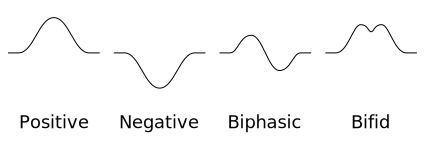
\includegraphics{figures/intro/ecg_waveforms}
\end{center}
\caption[ECG Morphology]{
\label{fig:intro:ecg:waveforms}
A schematic representation of P- and T-wave morphology.
From left to right, a positive, negative, a positive--negative biphasic and a
positive bifid wave are shown.
}
\end{figure}

The terminology used to describe ECG waves is illustrated in
figure~\ref{fig:intro:ecg:waveforms}.
Positive waves, those with a deflection above the baseline, and negative waves,
with a deflection below the baseline have already been explained.
The P- and T-waves can have more complex morphology however.
A P- or T- wave which shows both positive and negative deflections is termed
biphasic.
A positive--negative biphasic deflection is one which is first positive and then
negative.
A wave for which the converse is true is called negative--positive.
A wave which is entirely positive, or negative, but that has a notch in the
middle is described as bifid.

\subsection{The Vectorcardiogram}

Orthogonal lead systems, intended to measure the three independent components of
the heart's dipole, were first proposed in the middle of the 20th century.
Frank~\cite{Frank1956}, after experiments on physical models of the torso,
proposed his `corrected' orthogonal system.
This was corrected in the sense that the three lead vectors measured were
truly orthogonal and of equal magnitude in each of the three directions.
This included the influence of internal conductive regions and variability in
heart location.
The system uses 7 electrodes.
The three vectors chosen are X, a horizontal vector, positive to the left.
The Y vector is vertical and is positive towards the feet.
The Z vector is horizontal and positive towards the back.

\begin{figure}
\begin{center}
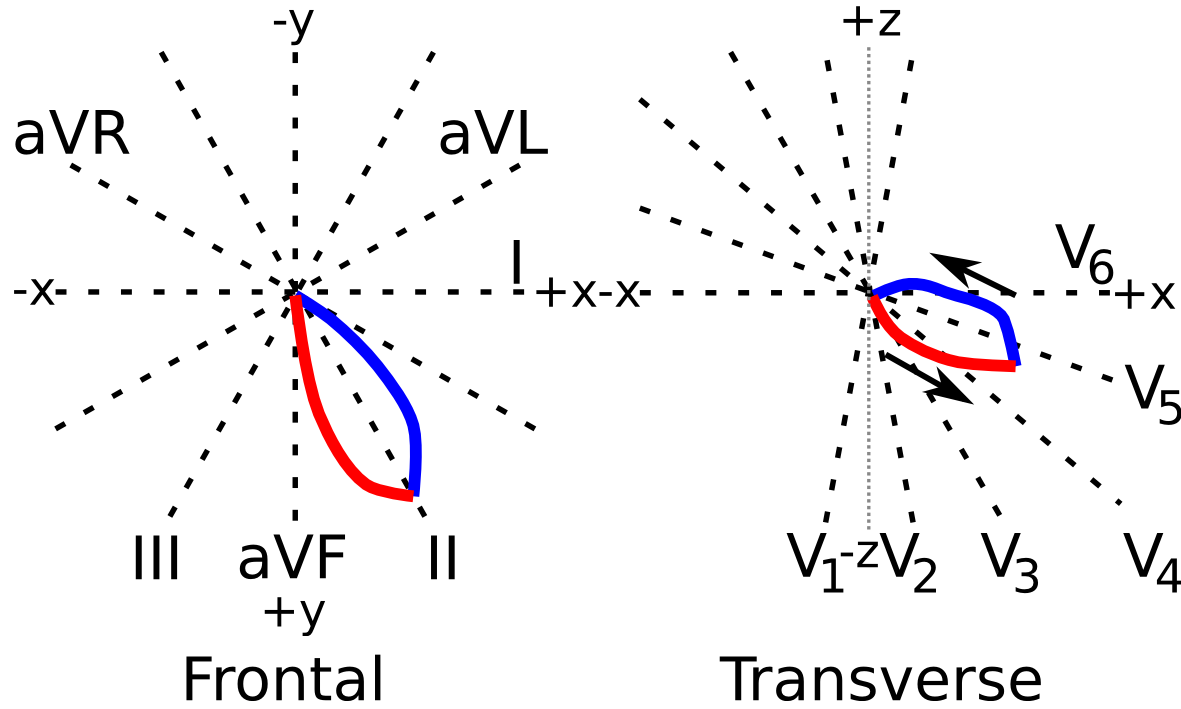
\includegraphics{figures/intro/vector_loops}
\end{center}
\caption[Schematic Vector Loops]{
\label{fig:intro:ecg:planes}
Schematic vector loops showing the relationships of the leads to the frontal and
transverse plane.
The lines of the leads are indicated in heavy-set black lines, the axes in grey
dots when they do not coincide with a lead.
The schematic loops are shown in red and blue, with arrows to indicate the
direction of inscription.
The afferent, or outgoing, limb of the loop is shown in red.
The efferent, or incoming, limb of the loop is shown in blue.
}
\end{figure}

The vectorcardiographic leads can be combined to visualize the electrical
activity of the heart in three planes.
These are the frontal plane, which combines Y and X, the transverse plane, which
combines X and Z, and the sagittal plane, which combines Y and Z.
The frontal plane is the one in which the limb leads measure, whilst the transverse plane
can be related to the precordial leads, as illustrated in
figure~\ref{fig:intro:ecg:planes}.

Dower~\cite{Dower1980}\ proposed a series of coefficients for the three Frank
leads that would convert the Frank leads into the standard 12 lead ECG.
However, the Frank leads are not recorded in common clinical practice.
To remedy this fact, Edenbrant and Pahlm~\cite{Edenbrandt1988} (and others, for
example~\cite{Uijen1988}), proposed an `inverse dower' transformation.
The inverse dower transform is a set of $8\times3$ coefficients
(table~\ref{tbl:intro:ecg:inverse_dower}) which are used to multiply the eight
independent components of the twelve lead ECG (I, II, $\text{V}_{\text{1--6}}$)
to form the three Frank leads.


\begin{table}
\caption[Inverse Dower Factors after Edenbrandt and Pahlm]{
\label{tbl:intro:ecg:inverse_dower}
Factors to construct the Frank VECG from the standard 12 lead ECG
set~\cite{Edenbrandt1988}.
Each of the 8 leads are multiplied by the given parameters to provide the
orthogonal Frank lead.
}
\begin{center}
\begin{tabular}{c c c c c c c c c}
\toprule
& $\text{V}_{\text{1}}$ &$\text{V}_{\text{2}}$ & $\text{V}_{\text{3}}$ &
$\text{V}_{\text{4}}$ & $\text{V}_{\text{5}}$ & $\text{V}_{\text{6}}$ & I & II \\
\midrule
X & $-0.172$ & $-0.073$ & $0.122$ & $0.231$ & $0.239$ & $0.193$ & $0.156$ & $-0.010$ \\
Y & $0.057$ & $-0.019$ & $-0.106$ & $-0.022$ & $0.040$ & $0.048$ & $-0.227$ & $0.886$ \\
Z & $-0.228$ & $-0.310$ & $-0.245$ & $-0.063$ & $0.054$ & $0.108$ & $0.021$ & $0.102$ \\
\bottomrule
\end{tabular}
\end{center}
\end{table}




\subsection{Body Surface Potential Mapping Arrays}

Body surface potential mapping arrays consist of many electrodes distributed
over the body and recorded simultaneously.
These allow the whole of the body surface potential to be examined and
to be used to establish diagnostic
criteria (for example, \cite{Dubuc1993,SippensGroenewegen1998}).
Mapping systems are also important for so called `inverse solutions', where the
cardiac sources are estimated from the external potentials (for example,
\cite{Ramanathan2006}).
They are also used for the construction of new lead sets (for example,
\cite{Sobieszczanska2007}).
Arrays of anywhere from 16 to over 200 electrodes have been used in such
studies.

\section{The Forward Problem}

The so-called `forward problem' seeks to find a relationship between the
electrical activity in heart and the potentials observed outside the heart,
most usefully on the surface of the body.
When looked at another way, it is a method of finding the lead field, $\vec{L}$,
for a given body.
The problem has been approached in a number of ways; experimentally, clinically
and numerically.

\subsection{Uses of the Forward Problem}

The original investigations into the forward problem very much concerned
themselves with finding $\vec{L}$.
They sought to refine the understanding of such concepts as the einthoven
triangle and the precordial electrodes and to more closely relate the differing
potentials observed with what was happening in the heart.
The experiments in the forward problem led to the lead field theory of McFee and
Johnson~\cite{McFee1953}\ and the Frank vectorcardiogram~\cite{Frank1956}.

Modern investigators of the forward problem use the solutions to perform similar
investigations, such as the development of new lead systems~\cite{Ihara2007}.
Forward solutions are also used for investigations into ischeamia, ventricular
and atrial fibrillation, conduction defects, amongst many.
Forward solutions also form the basis, or are used in the refinement, of inverse
solutions.

\subsection{A Brief History of the Forward Problem}

As has been mentioned, the initial uses of the forward problem were to determine
how the activity of the heart related to the leads.
These initial models tended to be real and physical models.
Towards this end, one of the first models constructed was by Burger and van
Milaan~\cite{Burger1946}, who constructed a one third life-size model of the
torso, filled with electrolyte solution.
The model had a cork spine and sandbags to represent the lungs.
The measurements from this model formed the basis for their refinements to the
lead theory.

Of the early mathematical models Brody~\cite{Brody1956}\ is one of the most
significant.
His was a model of the influence of the highly conductive blood masses of the
heart on the measured electrical field.
The `Brody Effect' is still used in literature today.

In the 1960s, numerical models of the torso started to
appear~\cite{Barr1966,Barnard1967}.
These initial models generally had a handful of dipoles, or even just one, to
represent the heart.
These were used to investigate the influence of dipole position and
heterogeneities on the body surface potential.

In 1971 Rush~\cite{Rush1971} published his torso model.
This was probably the ultimate torso model, literally and figuratively.
The model was twice lifesize and incorporated internal inhomogeneities
representing lungs, heart, heart blood, great blood vessels, liver, fat,
skeleton and anisotropic skeletal muscle--though the model could be used without
them as well.
The cardiac activity was represented by a number of dipole sources which were
located in the heart region of the torso.

In the 1980s, models of the heart and the torso gained more
sophistication~\cite{Gulrajani1983,Horacek1987}, though they were still generally
ventricular models, not models of the whole heart.
Models of this era routinely used 10s of dipole sources.
These models still did not include even primitive electrophysiology models,
although towards the end of the decade, propagation of the excitation wavefront
was being modeled~\cite{Aoki1987}.

Moving to the nineties and the turn of the millenium, the availability of
medical imaging tools such as CT and MRI scans allowed more accurate models to
be constructed~\cite{Weixue1993,Weixue1996}.
This is also when the first models began to appear which incorporated the
atrium~\cite{Weixue1996,vanDam2005}.
Many of the models published in this era use myocyte models to simulate the
propagation, some even using biophysically detailed models.

\subsection{Numerical Approaches}
\label{sec:intro:forward:numerical}

Numerical solutions to the forward problem involve solving Maxwell's equations
within the torso.
The same assumptions which were made for the lead field theory
($\S$\ref{sec:intro:ecg:lead_theory}) are valid here.
To reiterate them briefly, they state that the body is a linear volume
conductor.
There are no inductive or capacitive effects.
Furthermore, due to the finite (and small) size of the body, there are no
propagation effects to consider.
The field in the body, $\vec{E}$ is therefore given by
\begin{equation}
\label{eqn:intro:forward:maxwell}
\vec{E} = -\nabla\phi
\end{equation}
where $\phi$ is a scalar potential field.
Current flow in the torso under these conditions is given by Ohms law, which
states the total current flow, $\vec{J}$, is
\begin{equation}
\label{eqn:intro:forward:ohm}
\vec{J} = \mathbf{\sigma}\vec{E} + \vec{J^i}
\end{equation}
where $\mathbf{\sigma}$ is the conductivity tensor and $\vec{J^i}$ is an
impressed, or applied, current density which is generated by active sources,
i.e. the heart.

Since the total current flow is solenoidal, i.e. the net current flow into and
out of a volume is zero, via (\ref{eqn:intro:forward:ohm}) we have that
\begin{equation}
\label{eqn:intro:forward:ohm2}
\nabla\cdot\vec{J} = 0 = \nabla\cdot\left(\mathbf{\sigma}\vec{E} + \vec{J^i} \right)
\end{equation}
This can alternatively be written as
\begin{equation}
\label{eqn:intro:forward:poisson}
\nabla\cdot\vec{J^i} = \mathbf{\sigma}\nabla^2\phi
\end{equation}
If the body is homogeneous and isotropic, it becomes
\begin{equation}
\label{eqn:intro:forward:poisson2}
\nabla^2\phi = \frac{\nabla\cdot\vec{J^i}}{\sigma}
\end{equation}
which is Poisson's equation.

Finding $\phi$ for a given $\vec{J^i}$ can be achieved using a volume or
boundary based approach.
Volume based approaches \cite{Seger2004,Klepfer1997,Keller2007}\ involve dividing the body
up into volumes of different conductivity.
There is also the recent `Meshless Finite Element Method'~\cite{Li2007a}, which
uses the nodes of a typical finite element method, but not the elements.
The solution for $\phi$ is found using a finite element or finite difference
method.
Boundary element based approaches
\cite{Barr1966,Clayton2002,Gulrajani1989,Weixue1996}\ divide the torso into
regions of isotropic and uniform conductivity.
The potential, $\phi$, is found on the surfaces of these regions.

Volume based methods allow for a more complex model.
Interior volumes can have internally varying or even anisotropic conductivity.
They tend to be much more computationally intensive to solve, however, because
the problem space is still three dimensional.
In addition, the required element size can be quite small, especially for finite
difference approximations.
Keller~\cite{Keller2007}\ used a model with more than ten million torso
elements, for example, whilst the finite element model used by
Klepfer~\cite{Klepfer1997}\ has approximately one million elements and 168,000
nodes.

Boundary element based methods by contrast tend to be much simpler to solve.
Typical model sizes are of the order of a thousand to ten thousand elements, as
they reduce the problem space to a series of two dimensional surfaces.
This reduces the computational effort required.
However, since the solution is only computed at the surfaces, regions can only
be uniform and isotropic.






\section{A Cardiac Simulation Toolkit}

Cardiac simulation toolkits have existed in one form or another for some
time and include both commercial and open source 
Several cardiac simulation systems have previously been released, one of
the first of which is the OXSOFT HEART~\cite{Noble-1999}.


%    \chapter{Constructing a Cardiac Simulation Toolkit}

\section{Simulation Environment}

The simulation environment provided by the cardiac toolkit is intended to be as
portable as possible, so that numerical experiments may be run on whichever
platforms are appropriate.  To this end, all the data input structures are based
on open standards, or simple binary formats.  The output formats provided by the
various driver programs are also in simple binary or ASCII formats, to allow
them to be easily visualized with both commercial and open source visualisation
tools.  The results presented later in this chapter were performed on desktop
computers with a XX GHz Althon X2 chip and 1 GB RAM and on Horace, the local HPC
facility.  Horace has 24 compute nodes, each one consisting of four Intel Itanium2
Montecito Dual Core 1.6GHz processors, 16GB RAM and up to 512GB of local scratch
space.  The nodes are connected by a high speed Quadrics QsNetII
interconnect~\cite{horace}.  Horace provides compilers for both Fortran and C,
and for both the MPI and OpenMP parallelization libraries.

\subsection{Implementation}

The experimental protocol drivers and the cellular models were implemented in
the C programming language, although much of the supporting code and
supplementary tools were implemented in the ruby programming language.  The
cellular models currently implemented are based on the Hodgkin-Huxley formalism,
although there is no fundamental reason why a Markov chain based model could not
be included.  Inter-cellular coupling for propagation of excitation over a
strand or tissue was implemented using the monodomain equations.

\subsubsection{Cellular Models}

The cellular model used for much of the developmental process was the
Courtemanche et al. human atrial myocyte model~\cite{crn98}.  Also currently
implemented are the Nygern et al. human atrial myocyte model~\cite{nygern98} and
the four variable formulation of the Fenton-Karma minimal variable
model~\cite{overo2008}.  These cellular models describe the behaviour of a cell
using coupled systems of non-linear ordinary differential equations.  The ODEs
represent the concentrations of intra- and extra-cellular ion species and the
flow of current through ionic channels in the cell membrane or between
intra-cellular compartments, or their notional equivalents in the case of minimal
variable models.

These equations were generally solved using the simplest time-stepping method
available, the explicit Euler method.  To improve performance and stability,
some variables were integrated using the Rush-Larsen method.  More complex
integration schemes were tried, but did not significantly improve performance to
compensate for the greater complexity.

\subsubsection{Monodomain Equations}

The monodomain equations were used to couple multiple cells together to describe
a tissue over which excitation could be conducted.


A discussion of the merits of the monodomain and bidomain equations can be found
in the introduction.


\subsubsection{Strand Model}

The 1D strand model is used for several experimental protocols, as
a computationally cheaper alternative to a full tissue model.  The 1D strand
model consists of a number of nodes, typically 200 or 300, which are coupled
electrically at the ends of the cells.  The electrical activity at each node is
modelled via a cellular electrophysiology model and electrical conduction between the
nodes is handled via a 1D formulation of the monodomain equations, with no
flux boundary conditions.

\subsubsection{Sheet Model}

The 2D sheet model is used for several experimental protocols, as well as more
general numerical experimentation.  The 2D sheet model consists of a grid of
nodes, coupled electrically along the cardinal directions of the grid.  The
electrical activity at each node is modelled via a cellular electrophysiology
model.  Conduction of the electrical excitation between the nodes uses the
mono-domain equations with no flux boundary conditions applied at all tissue
boundaries.  The square sheet model, used in several of the numerical
experimental protocols described later, is typically 375x375 nodes, representing
140625 cellular models.  Two dimensional idealizations of physiological
preparations can have many more nodes, to on the order of $10^{6}$ cellular
models.  These idealizations can often be quite irregular and so to allow easy
and effective partition of workload across multiple processors, the tissue map
is decomposed into a 1D array which contains references to the neighbouring
cells.


\subsection{Parallelization}

Some parts of the toolkit require the modelling of large numbers of cells, on
the order of tens or even hundreds of thousands of cellular models in two
dimensional sheets.  Solving all the equations involved takes a significant
amount of time and so it is desirable for such simulations to be parallelized so
that the work involved can be split over several processors.  This can have
advantages beyond merely having eight rather than one cores worth of
computational cycles working on solving the equations.  Splitting the work over
multiple cores can also increase the amount of cache available, allowing for
more efficient operation of the solvers.

For the toolkit, the OpenMP~\cite{OpenMP} parallelization library was chosen.
This implements the shared memory parallelism paradigm.  Using the shared memory
paradigm is simpler, due to the lack of explicit communication calls, and can be
faster, as there is merely memory access involved, rather than communication
over an network or other interconnect.  Finally, a program written using OpenMP
can, with some care, also be compiled serially if an OpenMP compiler is not
available.  Whilst a program implemented using a non-shared memory paradigm,
such as using the MPI library, would allow it to be executed on potentially more
processors which would potentially offer faster run times, in practice the eight
core shared memory system Horace provides as a compute node was general found to
be sufficient for the task.

\subsection{Optimisation}

The toolkit uses several techniques to optimize the computations performed,
reducing the number of processing cycles required to compute the results needed
for publication.  These optimisations are generally built around the principle
of ``No code is faster than no code'', although it might be more accurate to say
``No code execution is faster than no code executed''.  To explain this idea
another way, it is that no combination of compiler flags can compete with a
sensible choice of algorithm which minimizes the number of computational steps
to be performed or the amount of data to be written to a file.  This is not to
say that the compiler is are unimportant, but that it is merely the start of
optimisations, rather than the final step.

\subsubsection{The Compiler}

The toolkit has been compiled using the GNU C compiler (gcc)~\cite{gcc}, the
Intel C compiler (icc)~\cite{icc} and the Sun microsystems .  All three have
OpenMP implementations available and all three are capable of performing a
number of optimisations, controlled via flags.  The most important aspect of the
optimisations is that they should not alter the behaviour of the floating point
handling, as this could have significant impact on the final result computed.
Despite this caveat, the results of applying certain optimisation flags can be
quite significant.

\subsubsection{Caching of Computed Values}

Moving beyond the compiler, one of the simplest forms of optimisation is to only
calculate each value once, if at all possible.  This can be done in a number of
ways and the toolkit developed here implements two such methods for saving
computational time.

State saving is one of the most direct ways of caching computed values.  At a
particular point in the simulation, all of the state variables of the
system are copied into an intermediate location.  This might be a file on disk or
to another location in memory.  If the state is written out to a file, that file can
be used as a `save point', allowing the simulation to be continued from that
point in the future, ensuring work is not wasted.

When copied to another memory location, this allows the program to return to
that point in the future.  This is useful in modelling many experimental
protocols, which often call for a number of `conditioning' pulses to allow the
cell or model to settle.  The state can be saved after the conditioning pulses
and then the actual tests can be performed quickly, saving the execution of
several seconds of simulated activity.  This technique should obviously only be
used for cells in the Hodgkin-Huxley formalism which are deterministic and thus
give identical results whether the state is saved or not.  Using such a
technique with a cell that has a number of stochastic components could
potentially affect the quality of the results.

The second way in which caching can be employed is in the creation of `lookup
tables'.  A lookup table is a pre-computed table of the values an expression can
take.  When the expression would normally be evaluated, the table is used
instead, replacing what might be a complicated expression with a single array
lookup.  For lookup tables to be efficient to pre-compute, the tabulated
expression should depend on only one variable and should be sufficiently
`complex' expression, such as one involving the computation of mathematical logs
or exponentials.  The expression should depend on only one variable as the
pre-computed table has to be indexed over each variable the computation depends
on and even dependence on just two variables would increase the number of table
entries required by thousands or millions.  The requirement for complexity is a
little more obvious, as any optimisation can only save as much time as the
original series of operations took.  With these limitations in mind, it is still
possible to find many candidates for pre-computation in typical cardiac cell
models, most notably the activation and inactivations of voltage dependent
gates.  This technique is typically only worthwhile performing in the case of
tissue simulations where the benefits can be shared amongst all the cells since
pre-computation can be quite expensive, destroying any efficiency gains made
through their use for single cell simulations.

\subsubsection{Binary Searches}

Several of the experimental protocols provided by the toolkit are intended to
determine the value of a parameter which causes a particular condition to be
fulfilled, such as a successful excitation of the cellular model after
progressively shortening stimulus intervals.  This value we will call the
critical value. In real experiments, ones involving actual cardiac tissue, the
typical experimental protocol would involve stimulating the tissue at
sequentially shorter intervals, until no stimulation was provoked.  This might
involve stimulating the cell thousands of times, which would be expensive
computationally to model exactly.  Instead, a binary search for the critical
value can be performed, using the pseudo-code shown here.


To explain in words, first two guesses are made; the high guess, which is the
maximum value that the critical value can take, and the low guess, the minimum
it is presumed to take.  The simulation is then run with the parameter set at
the average of the low and high guesses--the current guess.  If the test is
successful, the critical value evidently lies somewhere between the low guess
and the average, and so the high guess is set to the current guess.  Conversely,
if the test is unsuccessful, the critical value is obviously above the current
guess, and so the low guess is set to the current guess.  The simulation is then
repeated with the average of the new high and low guess.  Using this algorithm,
the search space is halved with each iteration, swiftly finding the critical
value.  For example, to find a parameter somewhere in the range of 0--1000~ms to
the nearest millisecond requires just 10 iterations of the binary search
algorithm, but might take hundreds of iterations with sequential searching.

One important thing that must be considered when using binary searches is that
there is only one critical value in the range considered or else the algorithm
will give unpredictable results.  In practice, this limitation is often quite
easy to work within.

\subsubsection{Adaptive Step}

Adaptive step mechanisms are employed in the toolkit when there is a need to
provide output over a wide range of times, when the slope of the graph is not
constant over the range to be graphed.  This is very common in the modelling of
cardiac cells, which often show an exponential dependence of various parameters
on the  stimulus interval, and are graphed over a range of hundreds or thousands
of milliseconds.  A step that sufficient to track the curve at the upper limits
of the range will completely fail at the steeper slow of the lower limits,
whilst a step that will track the curve for the lower limits will result in
unnecessary work being done at the upper end of the range.  To alleviate this
problem, an adaptive stepping mechanism is used, as shown in this pseudo-code.

First, the measurement is performed at the largest desired point.  The interval
is then reduced by the step, and the measurement is performed again.  The
difference in the measurements is calculated and compared to the desired maximum
delta.  If the difference is acceptable, the interval is once more reduced by
the step, and the measurement taken once more.  If the difference is too great,
then instead the step size is halved and the measurement repeated.  If the
difference is now acceptable, then the interval is reduced by the new step and
the experiment proceeds.  If it is not, then the step size is once more halved.
The step size used is therefore always appropriate to the slope of the curve and
a smooth graph results.  Additional logic, not shown in the pseudo-code, is used
to ensure the step size does not become too small, and to terminate the graph at
the lower end of the range.

Since curves can increase or decrease the absolute difference between the two
values is compared.

\subsubsection{Parallel Input/Output}

Input and output for simulations is obviously essential if they are to be of any
use.  This input and output can involve the reading or writing of many megabytes
or gigabytes of information over the course of a simulation, often in a variety
of different formats.  This most significant for sheet simulations and it is
those that we consider here.

Data input is typically not that significant a cost for
simulations, as whilst various simulation maps and saved states be quite large,
the cost is typically only paid once.  Data output is often required at numerous
points throughout the course of the simulation since almost all simulations are
performed to examine the time evolution of the cardiac system.  Many simulations
will output the value of state parameters, most commonly the voltage, at all
points in the tissue every few milliseconds of simulated time.  Other state
variables might also be desired and the toolkit also offers `live visualization'
of two dimensional sheets via output of images in the GIF format.  In addition,
the whole state is output regularly, to allow simulations to be resumed at a
later point in time.  This output usually stops all simulation whilst it is
being written to disk, time during which the processors are typically idle.  By
allowing multiple threads to output in parallel, the cost of outputting multiple
files can be reduced to the cost of outputting one.


\section{Experimental Protocols}

The toolkit developed provides a number of experimental protocols to use with
the cellular models to quantify the electrophysiological behaviour of the
modelled cells.  The provided protocols include the action potential duration at
90\% repolarisation (APD90) and the action potential (AP) profile; the
APD90 and APD50 restitution; the effective refractory period (ERP) restituion
(ERPr); the conduction velocity (CV) restitution (CVr); the temporal
vulnerability window to unidirectional conduction block (VW) and a flexible
system for specifying two dimensional sheet experiments, including the
initiation of re-entry via wavebreak protocols and computation of the spatial
vulnerability window.

\subsection{Action Potential Duration}

\subsection{Action Potential Duration Restitution}

The toolkit calculates the APDr via a standard S1--S2 protocol used in both
numerical simulations and also in physiological experiments.  The APDr is used
as a measure of how the cell responds to stimulations at different rates.  The
protocol used is shown here.


The cellular model is paced nine times with a stimulus close to the threshold
value at a given frequency or BCL.  At this point, the state is saved for the
paced cells.  The tenth S1 stimulus is then given, followed by the S2 after a
varying DI, which is reduced via an adaptive step to record the relationship
between DI and the APD of the following AP.  The toolkit also determines useful
parameters such as the maximal slope of the restitution curve, which can be
related to the stability of spiral waves within the tissue.  Both the APD90 and
the APD50 restitution can be calculated.

\subsection{Effective Refractory Period Restitution}

The ERPr is calculated by the toolkit using standard experimental protocols.
The ERP is defined as the shortest possible stimulus interval, $S2$, which still
allows a successful AP to be elicited after pacing $N$ times at a pacing
interval $S1$.  A successful AP is defined as an AP which has an amplitude
of at least 80\% of the magnitude of the preceeding AP.  To determine the rate
dependence of the ERP, it is evaluated at a decreasing $S1$ interval.

To find the ERP for a given $S1$ interval the cellular model is paced $N$ times
at that interval. The state is saved just before the $N-1$th AP is initiated.
The ERP is found via binary search.  The low guess for $S2$ is typically chosen
as zero, whilst the high guess is the $S1$ interval being tested.  The $S2$\
interval for each attempt is the average of the high and low guesses.  After the
state has been saved, the $N$th AP is initiated and its amplitude recorded.
Then \ms{S2} after, the test AP is invoked.  If it is successful, that is if it
has an amplitude of at least 80\% of the magnitude of the $N$th $S1$\ AP, then
various parameters relating to the APs are stored such as the $S1$\ and $S2$\
amplitudes and the ratio between them.  The stored state is then restored to the
cellular model and the next binary iteration is attempted, until the ERP has
been found at the desired precision.

The reduction in $S1$\ interval is stepped via an adaptive mechanism which is
used to keep the reduction in ERP between successive $S1$ intervals to below
\ms{1}.  The $S1$\ interval is reduced until it is sufficiently short that the
$S2$ interval would fall within the $N$th AP.

\subsection{Vulnerable Window}

The VW is principally a tool of numeric experimentation, based around a 1D ring
model of cardiac arrhythmia.  The VW is defined as the time period after a
stimulation during which a second stimulus elicits unidirectional propagation
along the strand.  In the case of a ring this causes retrograde propagation
which cycles endlessly.  If the stimulus is given too early, then the tissue
will still be refractory and no propagation of excitation will ensue.  If it is
given too late, then propagation will occur in both directions, which in the
ring case, results in the two excitation wavefronts annihilating each other.
Normal pacing could then resume.

The VW is found in a 1D strand model, set up as described previously.  The
strand is 200 units long and with a space step of \mm{0.1}.  The first stimulus is
given to a 3 unit (\mm{0.3}) section at one end of the strand.  The test stimulus
is given to a 4 unit (\mm{0.4}) section, usually centred in the middle of the
strand. The VW is bounded on the lower side at the time when a stimulus any
earlier would result in no propagation from a test stimulus, and on the upper
side at the time when a stimulus any later would result in bidirectional
propagation from a test stimulus.  These three cases (no, unidirectional,
bidirectional) propagation are illustrated in figure TODO.

By counting the number of APs which cross the two ends of the strand--2, 3 and
4, respectively, for the three cases in figure TODO--the result of the test
stimulus can be determined.  The two boundaries of the VW are found via binary
search, with a lower guess of \ms{0} and an upper guess of \ms{1000}.  First, the
upper bound of the VW is determined by searching for the delay when 3 APs
crossing the ends becomes 4.  The lower bound is then found by looking for the
delay at which 3 APs crossing the ends of the strand become 2.  A minor
optimisation is performed when looking for the upper bound, in that the lower
bound's high and low guesses are updated at the same time, reducing the total
space which must be searched in the second half of the program.  Before the test
stimulus is administered, the strand may be pre-paced a number of times.  In
this case the strand state is saved as the middle of the strand is depolarized
and then restored for each binary division.

\subsection{Threshold of Excitation}

The threshold of excitation is a theoretical measure, proposed by Zhang et
al.~\cite{Zhang2003}\ and used in modelling studies~\cite{Kharche2008}.  It is
defined as the minimum stimulus current which, when delivered to a cell, will
cause the cell to depolarize to a membrane potential of at least \mv{-20}.  The
threshold of excitation is calculated for a range of stimulus intervals,
successively reducing the interval until it is impossible to elicit a
depolarization of sufficient magnitude.  At each stimulus interval it is
recorded if the test pulse elicits bidirectional, unidirectional or no
propagation.

The threshold of excitation is found in a 1D strand model.  The strand is 300
units long, with a space step of \mm{0.1}.  The strand is first given $N$ S1
stimuli at a rate which allows the strand to recover between each excitation
wave.  Each S1 stimulus is delivered to the first 4 nodes (\mm{0.4}) and is
chosen to be above the threshold of excitation.  The threshold of excitation is
calculated at the 100th node and so as this node depolarises, the state for the
whole strand is cached.

The threshold of excitation is then found via binary search, with a lower bound
of \unit{0}{nS} and an upper bound chosen to be 5x the normal threshold.  The
test stimulus is delivered $\Delta t$\ seconds after the 100th node depolarises
to a group of 4 nodes centred on the 100th node.  After the test stimulus is
delivered the 4 nodes are tested for the excitation condition, attaining a
membrane potential of \mv{-20}.  If it is successful, the current stimulus
strength will assigned to the high guess.  If not, to the low guess.  In
addition, the simulation is continued to evaluate whether bidirectional,
unidirectional or no conduction of the excitation wave is evoked by the
stimulus.  The strand is then reset to the cached state and the new stimulus
strength is tested until a sufficient accuracy has been attained.  Once the
threshold of excitation has been determined for a given $\Delta t$\ the state of
the strand is once more reset to the cached state and a shorter $\Delta t$\
tested.

\subsection{Conduction Velocity Restitution}

Measurement of CV (or solitary wave velocity) itself is performed both
experimentally and numerically, as is the minimum conduction interval, which is
the shortest interval between an S1 and an S2 stimulus which still travels the
length of the strand.  This is similar to the ERP, but can also be influenced by
factors which affect the inter-cellular coupling as well as heterogeneity in the
strand.  The CV\emph{r} provides both the solitary wave velocity, the CV for a large S2
interval and the minimum stimulus interval, when the S2 interval gets too short
for an excitation wavefront to be fully propagated.

The CV\emph{r} is found in a 1D strand model, set up as described previously.
The strand is 300 units long with a space step of \mm{0.1}.  Stimuli are
delivered to a 4 unit (\mm{0.4}) length at one end of the strand at a strength
above threshold.  The strand is first given $N$\ S1 stimuli at rate which allows
the strand to recover between their application.  The S2 stimulus is then
delivered $\Delta t$\ seconds later. The conduction velocity is estimated from
the time taken to propagate between two points 100 nodes from each of the ends
of the strand, to minimize the influence of boundary effects.  The S2 time is
then stepped via an adaptive step, until a second excitation wave does not
propagate the length of the strand.


\subsection{Spiral Wave Life Span}

Spiral Wave LS is examined experimentally and numerically.  The LS of the spiral
wave and the meander pattern of the tip are both used to gain insight into the
behaviour of the tissue under conditions of cardiac arrhythmia.

Spiral waves are initiated in a square sheet of tissue $375\,\text{x}\,375$
nodes in dimension with a space step of \mm{0.1}, as described previously.  The
tissue is first stimulated along one edge via a stimulus current applied to a
row of nodes extending the length of the tissue and 3 nodes (\mm{0.3}) in width.
The planar wave is then allowed to propagate over the tissue.  Some time after
the first wave is initiated, a second stimulus is applied.  The second stimulus
is applied to half the tissue, bisecting the first wave's propagation front.
The second stimulus is a voltage clamp, with all the included tissue clamped to
a `high' potential, typically \mv{+20}--\mv{+50} for a millisecond.  The
generated spiral is then allowed to evolve until it self-terminates, the spiral
wave tip exits the tissue or until a sufficient amount of time has passed such
that the spiral can be classified as `persistent'.  The time allowed for a wave
to be classified as persistent is typically 5 or \unit{10}{s}.

The spiral wave tip traces are calculated via a standard contour based
algorithm, comparing the \mv{-60} contour line on snapshots of the electrical
activity \ms{2.5} apart.

\subsection{Spatial Vulnerability Window}

The SVW is examined both experimentally and numerically.  It is used together
with the (Temporal) VW for quantifying a mutation or condition's potential for
arrhymogenesis.  It is defined as the smallest area of tissue in a 2D sheet,
which when given a threshold stimulus in the wake of a conditioning pulse causes
at least one `figure of eight' re-entry.  A figure of eight re-entry occurs when
the excitation waves from the tips of the test area propagate back through the
centre of the area, resulting in a pair of contra-rotating spiral waves at each
end of the region.

The sheet model used for the determination of the SVW can vary in size, as the
SVW can vary substantially, depending on the electrophysiology being simulated
by the cellular models at the nodes, but the smallest used is typically
$375\,\text{x}\,375$ nodes, with a spatial resolution of \mm{0.1}.  The sheet is first given one
conditioning excitation, initiated by injecting a strip of nodes 3 nodes
(\mm{0.3}) in width with current along one edge of the sheet.  The wave is then
allowed to propagate through the tissue.  When the VW of the tissue is
positioned at the centre of the tissue, the test stimulus is delivered.  The
test stimulus is an area of tissue 20 nodes (\mm{2}) wide and of variable length.
After the test stimulus is delivered, the sheet is observed until figure of
eight re-entry is observed, or it is obvious that it will not occur.  The
protocol is then repeated with a test stimulus area of greater length.


\section{Results From Simulation Studies}

The cardiac simulation toolkit has been used in several simulation studies.
Here I present two such studies, representing different aspects of the toolkit.
The first is based on an experimental study which determined the existence of a
novel ion channel in the human atrium which caries an anion current through the
cellular membrane.  The second is principally a 2D study, concerning the effects
of Atrial Fibrillation induced Electrical Remodelling (AFER) and
electrophysiological heterogeneity in a 2D idealization of the right atrium and
the sino-atrial node.

\subsection{Anion Currents In The Human Atrium}

\subsubsection{Introduction}

In a recent experimental study, Li et al.~\cite{li2007} determined the existence
of a novel outwardly rectifying anion current in human atrial myocytes isolated
from right atrial appendages taken from patients undergoing coronary bypass
surgery.  They determined that it was separate other known ionic currents and
performed preliminary modelling based on the CRN Human Atrial Myocyte
model~\cite{crn98}.  They determined the current could be modelled by
equation~\ref{anion:eqn} with the constants given in table~\ref{anion:table}.

The total current carried by the channel, \ii{ANION}, was given by

\begin{equation}
\label{anion:eqn}
I_{ANION} = g_{ANION} \frac{V-E_{ANION}}{1-\left(c\times e^{\left(V-E_{ANION}\right)}\right)}
\end{equation}

where $g_{ANION}$ is the conductivity of the anion channel, $E_{ANION}$ is
the reversal potential of the channel and $c$ and $d$ are constants to
describe the behaviour.  All other symbols have their usual meanings.

\begin{table}
    \caption[Parameter sets for the anion sensitive current]{
        Parameter sets for the anion sensitive current \ii{ANION}\ when carrying
        \nothree\ and $\text{Cl}^{\text{-}}$\ ions.
    }
    \begin{tabular}{ l  c c}
    \label{anion:table}
    & \nothree & $\text{Cl}^{\text{-}}$ \\
    \hline
    $g_{ANION}$ & 0.37   & 0.19 \\
    $E_{ANION}$ & -45.64 & -45.64 \\
    $c$         & 0.87   & 0.94 \\
    $d$         & $8.4\,\text{x}\,10^{\text{-4}}$ &  $2.5\,\text{x}\,10^{\text{-4}}$
    \end{tabular}
\end{table}


The simulation study used the parameter set for the anion current carrying
\nothree ions.  The effects of the addition of this current to atrial
myocyte cells was quantified .  In the following
paragraphs, `control' is used to denote the unmodified CRN model and `anion' to
denote the CRN model with the additional current described by (\ref{anion:eqn})
with the \nothree\ parameter set from Table \ref{anion:table}.

\subsubsection{Methods}

The effect on the behaviour of the cells caused by the introduction of the anion
current was quantified using the simulation library described previously in this
chapter for control (no \nothree-sensitive \ii{ANION} current) and anion
(\nothree-sensitive \ii{ANION} current present) cases.  As this simulation study
was based on the CRN cell, the standard stimulus was \ms{2} in duration and
\unit{2}{nS} in magnitude.  Unless an alternative protocol is mentioned, all
simulations directly followed those set out at the start of this chapter.  None
of the simulations presented in this section involve the use of lookup tables of
voltage dependent properties.

Simulating a single cell, the following measures were quantified: the AP
profile, the restitution of APD at 50\% repolarization, \apdr[50], the
restitution of APD at 90\% of repolarization, \apdr\ and the Effective
Refractory Period restitution, ERP\emph{r}.  The maximal fast sodium activation
was quantified at the same time as the \apdr\ was computed and is the product of
the three gates in \ii{Na}, as $m^{3}hj$. In all the single cell cases, the
cell was paced 10 times before the measurement was taken, to allow simulation
parameters to settle and to adapt to any changes in pacing rate.  Storage of the
cellular state was used in all appropriate points in the simulation, to minimise
computational time.

Using a 1D strand model the temporal Vulnerability Window to unidirectional
conduction block, VW, the Conduction Velocity restitution, CV\emph{r}\ and the
threshold of excitation were computed.  The strand model used was 300 nodes long
and had a space step of \mm{0.1}.  The diffusion coefficient, $D$, was set to
$0.03125\,\text{mm}^{\text{2}}\,\text{ms}^{\text{-1}}$~\cite{Biktasheva2005}.
In all 1D simulations the strand was paced 10 times before measurement was
taken.  In all simulations this state was then cached and restored as
appropriate, as described in the algorithms section of this chapter.

Using a 2D tissue model the lifetime of re-entrant spiral waves was estimated,
following the wave-break protocol outlined earlier.  The sheet had dimensions of
$375\times375$ nodes and a space step of \mm{0.1}.  The clamp potential used
to break the wave was \mv{+50} and it was applied for \ms{1}.

\subsubsection{Results}

The AP generated by the control and anion simulations are shown in
figure~\ref{anion:ap}.  The \apd\ is relatively unchanged, but is slightly
reduced from \ms{299.6} to \ms{298.0}, whereas the \apd[50]\ is significantly
reduced, from \ms{180.1} to \ms{160.1}.  The AP profile shows a depressed plateau region (phase
2), reduced from \mv{-9.56}\ to \mv{-14.1}\ and a slightly elevated resting potential,
\mv{-79.0}\ in the anion case cf. \mv{-80.9}\ in control.  This duplicates the Li et
al.~\cite{li2007} study, and is included here only for completeness.

\begin{figure}
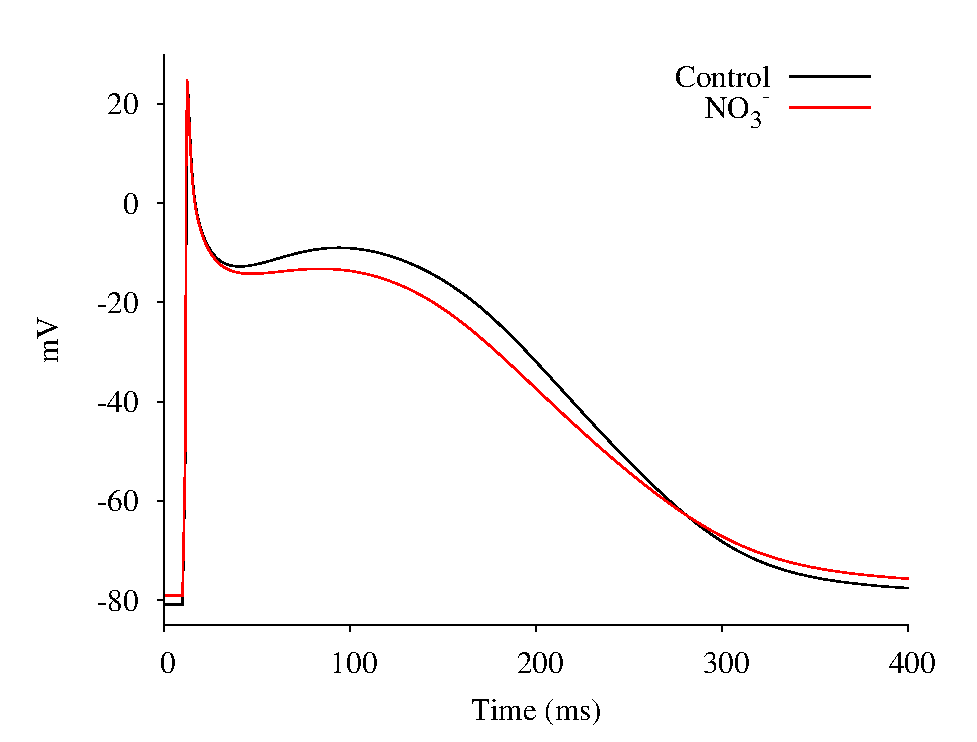
\includegraphics{figures/toolkit/anion/01_AP}
\caption[Anion Sensitive AP Profile]{\label{anion:ap} AP profile for the CRN
model in control (black) and anion (red) cases.  The inclusion of the
\nothree\ carrying current results in a small change of AP morphology, with
a depressed plateau potential and an elevated resting potential.}
\end{figure}

The APD\emph{r}\ curves produced by the control and anion cases are shown in
figure~\ref{anion:apdr50} and \ref{anion:apdr90}, for the restitution of APD at
50\% (\apdr[50]) and 90\% (\apdr) of repolarization, respectively.  The
\apdr[50]\ shows the most significant differences, with the anion
curve depressed by \ms{20} even at the largest DI, increasing to a maximum
difference of over \ms{40} at at DI of \ms{380}.  The two curves then rejoin each
other before they cross over at a DI of \ms{200}.  The \apdr\ curves, by
contrast, are very similar for control and anion cases at large (over \ms{600}) DI.
Between \msrange{100}{400}\ DI, the anion case is depressed compared to the control
case, with a difference of up to \ms{25}\ observed in the measured APDs.  At
\ms{100}, the curves rejoin one another and show a rapidly increasing slope as the
DI approaches \ms{0}.

\begin{figure}
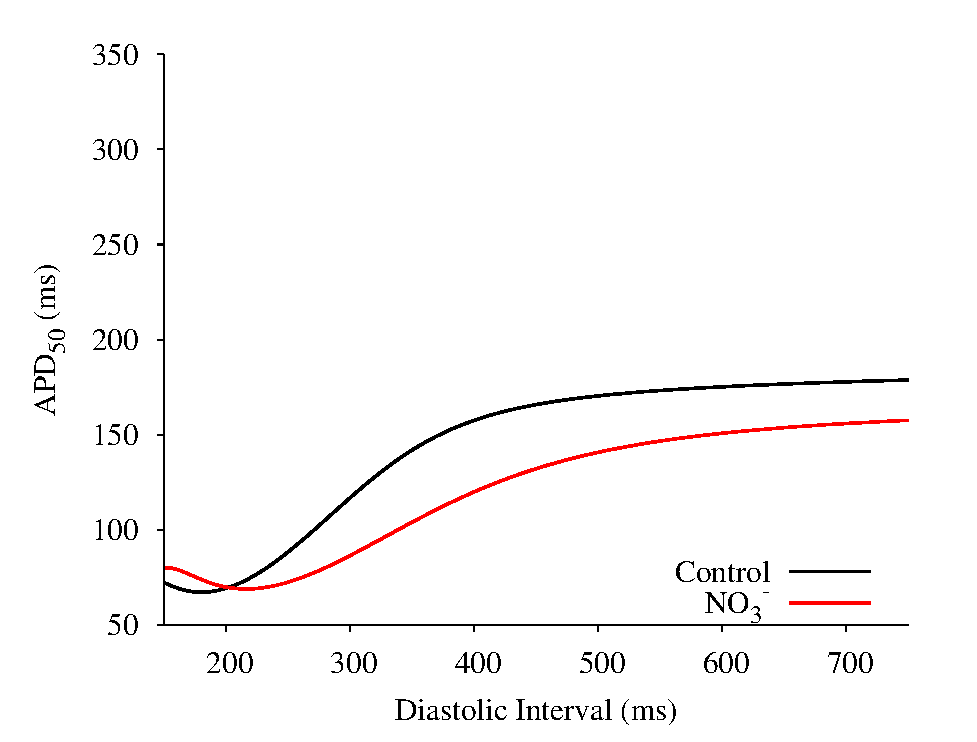
\includegraphics{figures/toolkit/anion/03_S1S2_50}
\caption[Anion Sensitive APD Restitution at 50 repolarization]{
\label{anion:apdr50} APDr curves for the CRN model in control (black) and anion
(red) cases at 50\% repolarisation.  The two variants are clearly different for
all the DI tried in the simulation, with the anion case considerably below the
control case for much of the DI tried.  The anion case also shows a reduced
slope of the restitution curve compared to the control case.  Note the
cross-over of the curves at a DI of \ms{200}.}
\end{figure}

\begin{figure}
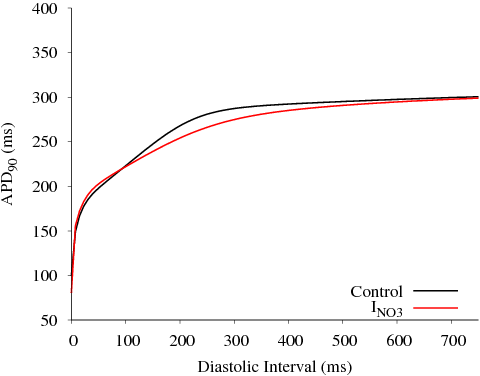
\includegraphics{figures/toolkit/anion/02_S1S2_90}
\caption[Anion Sensitive APD Restitution at 90 repolarization]{
\label{anion:apdr90} APDr curves for the CRN model in control (black) and anion
(red) cases at 90\% repolarisation.  The two variants behave the same at large
DI, but as the DI before the S2 stimulus is decreased, the anion case shows a
greater reduction in the \apd.  At short DI (below \ms{100}) the two curves
rejoin each other.}
\end{figure}

The ERP\emph{r} curves produced by the control and anion cases are shown in
figure~\ref{anion:erpr}.  In both cases the ERP\emph{r}\ curves are relatively
flat, decreasing by approximately \ms{60}\ over the \ms{700}\ range of S1
intervals considered.  The addition of the \ii{ANION}\ current changes the
behaviour of the ERP\emph{r} curve in a manner which is not simply a shift left
or right.  The control case shows a response which has a clear plateau region
which continues until an S1 interval of \ms{500}\ is reached and then a
relatively steeper decline until eliciting an AP of the appropriate magnitude
becomes impossible at an S1 interval of \ms{330}.  The anion case, by contrast,
shows a decreasing ERP over the whole range of S1 intervals considered although
it too shows its steepest slope just before eliciting a sufficiently large AP
becomes impossible, also at approximately \ms{330}.  At long S1 intervals (above
\ms{700}) the ERP\emph{r}\ is longer for the anion case before the curves cross
at \ms{600}\  and then again at \ms{450}\ with the ERP in anion at the point
where further stimulation becomes impossible almost \ms{20}\ higher than in the
control case.

\begin{figure}
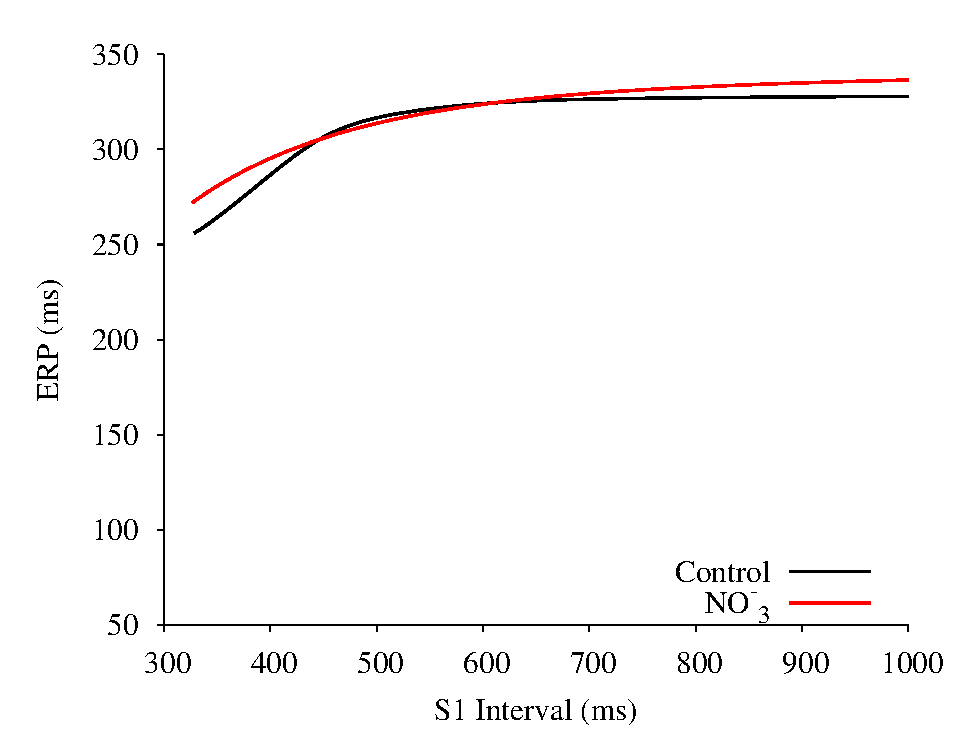
\includegraphics{figures/toolkit/anion/04_ERPR}
\caption[Anion Sensitive Effective Refractory Period Restitution]{
\label{anion:erpr} ERP\emph{r} curves for the CRN model in control (black) and anion
(red) cases.  The
addition of the \ii{ANION} current changes the behaviour of the cell from a long
and flat plateau region followed by a relatively sharp decrease into a more
constant decline.}
\end{figure}

The temporal VW increased with the addition of the anion current from
\ms{3.20} in
control to \ms{3.81}\ in anion case, a 20\% increase in the size of the region of
unidirectional conduction block.  The CV\emph{r}\ curves, shown in
figure~\ref{anion:cvr}, suggest that tissue with the anion sensitive current
shows faster CV at normal physiological stimulus intervals (corresponding to
\msrange{500}{1000}), with an average conduction velocity of
\cms{27.2}\ in anion, compared with \cms{26.9}\ in control.  As the conduction
interval is reduced below \ms{500}, the conduction velocity starts to decrease
rapidly until conduction stops at \ms{325} for anion and \ms{319} for control.
There is a brief recovery of conduction velocity visible in both cases, just
before conduction block.

\begin{figure}
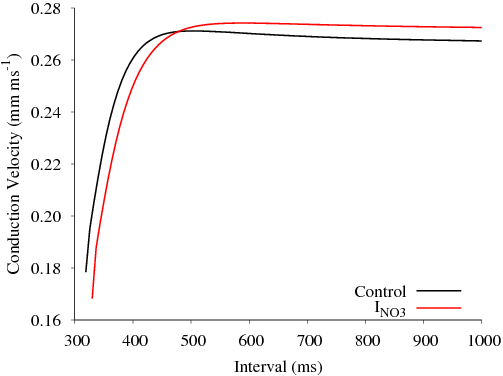
\includegraphics{figures/toolkit/anion/06_CV}
\caption[Anion Sensitive Conduction Velocity Restitution]{
\label{anion:cvr} CV\emph{r}\ curves for the CRN model in control (black) and anion
(red) cases. The CV\emph{r}\ curves are relatively flat for both cases over the range of
\msrange{500}{1000}, before they both increase rapidly in steepness until the minimum
stimulus interval is reached at approximately \ms{320} for both control and anion.
The CV is higher at longer stimulus intervals for the anion case, before it
crosses the control curve at a approximate stimulus interval of \ms{460}.}
\end{figure}

Spiral waves were induced in a square sheet.  Representative plots of the
membrane potential over the whole sheet, produced as the simulation was ongoing,
are show in figure~\ref{anion:spiral}.  Panels A i--iv show the membrane
potential for control, whilst Panels B i--iv show the membrane potential for
anion, as the simulation evolved.  The path followed by the spiral wave tip as
it meandered is shown in A,v and B,v for control and anion, respectively.  In
both cases the spiral wave starts in the centre of the tissue and then follows a
looping track around the tissue before finally it exits the tissue when it
cannot turn fast enough around its own refractory tail.  This process takes
\ms{1700} in control and \ms{2300} in anion.

\subsubsection{Discussions and Conclusions}

The effects of the inclusion of an anion sensitive current do not seem to be
that large, at least when considered on the single cell level.  This is perhaps
to be expected, as a current which did have a significant influence on the
action potential would surely have been identified sooner.  However, despite the
current's small influence on the action potential duration, it does have
significant effects on the restitution properties of the cell and on the
behaviour of cells in a tissue.

The most noticeable effect of the inclusion of \ii{ANION}\ in a cellular model
is the abbreviation of the \apd[50]\ and the accompanying reduction in the
plateau potential.  The abbreviation is due to \ii{ANION}\ acting as a
rectifying current when the membrane potential is above \mv{-45}.   Conversely,
at potentials below \mv{-45}\ \ii{ANION}\ acts to depolarize the cell, leading
to the slightly elevated resting membrane potential observed between action
potentials.  This difference in effect is what leads to the interesting
behaviours observed in cells with \ii{ANION}.

The \apdr[50]\ and \apdr\ curves show that \ii{ANION} has a rate dependent
effect.  Both curves are flattened in the cells which include \ii{ANION}\, but
this flattening is not uniform over the range of S2 intervals considered.
\ii{ANION}\ has a simple exponential dependence on the membrane potential and no
gating variables however, so it is not \ii{ANION}\ which causes this rate
dependence directly.  Instead, we must look to the currents active within the
plateau region of the action potential.  \ii{CaL}\ is the principle current
responsible for the plateau region of the action potential and unlike \ii{ANION}
it has both an activation gate, $d$, and an inactivation gate, $f$.  The $d$\
gate is not as interesting as the $f$\ gate, as its time-course is not affected
by the presence of \ii{ANION}, although its activation during the plateau region
is reduced.  Conversely, the $f$\ gate in \ii{ANION} cells never inactivates as
completely as it does in the control simulations which lack the current.

Considering next the 1D strand results, both the CV\emph{r} and threshold of
excitation data continue the story of a rate dependent influence.  At a long
stimulus interval, the increased excitability of the anion cells leads to a
higher conduction velocity.  The increased excitability at long stimulus
interval is due to the inward nature of the current in the very first stages of
the action potential.  This increased excitability allows the cells with
\ii{ANION}\ to conduct excitation faster until, at stimulus intervals of below
\ms{500}\ control cells start to conduct faster.  At this stimulus interval, the
threshold of excitation is still lower for the anion case, so another factor is
responsible for the reduction in conduction velocity.  The excitability of the
cell is an important influence on the conduction velocity, but it is not the
only factor.  Another major factor is the upstroke velocity which is principally
governed by the fast sodium current, \ii{Na}.  This is partially inactivated by
the elevated resting potential in the anion case, which also reduces the rate of
recovery of the inactivation variables.  When the test stimulus is delivered
after a reduced conduction interval in the anion case \ii{Na}\ does not open as
fully, slowing the upstroke and thus leading to a reduced conduction velocity at
short stimulus intervals, compared with the control case.  The increase in the
vulnerability window appears to be quite significant, an extra 20\% of the size
of the vulnerability window in tissue without \ii{ANION}.  Both the reduced
vulnerability window and the reduced conduction velocity at short pacing
intervals suggests that the addition of \ii{ANION} may be pro-arrhythmogenic.
The increased vulnerability window has an obvious influence on the genesis of
re-entrant excitation---A larger vulnerability window increases the chance of a
premature excitation interrupting the normal function of the heart.  The
influence of conduction velocity on re-entrant excitation is subtler, but a
reduced conduction velocity reduces the wavelength of the excitation wave.  This
allows a greater number of excitation waves to persist in the same area of
tissue, reducing the likelihood of a re-entrant excitation self-terminating.

Finally, considering the results from the sheet model of the tissue which was
used to investigate the lifespan of induced spiral wave re-entry, we can see our
hypothesis from the 1D strand results is born out.  A revolving spiral wave
typically rotates at a higher frequency than the normal excitation rate of
cardiac tissue.  The excitation waves in the 2D sheet are therefore operating in
the short stimulus interval regime.  Cells which contain \ii{ANION}\ have a
slower conduction velocity in this regime and so the spiral wave can be
sustained for longer due to it's shorter wavelength.  However, the reduction in
wavelength is not so severe as to create a stable mother rotor, as been observed
in studies of pathological conditions.

\subsection{Atrial Fibrillation Induced Remodelling And Heterogeneity}

\subsubsection{Introduction}

The human atria consists of several tissue types each with distinct
electrophysiological properties.  It has previously been shown that
inhomogeneity in tissues can lead to re-entrant activity
\cite{Bernus2005, Coronel1992, Kumagai1997}.  There is also experimental
data available on the ion channel remodelling due to atrial
fibrillation induced remodelling (AFER) during chronic atrial
fibrillation (AF) on human atrial cells~\cite{Bosch1999,Workman2001}.

In this study, we quantified the changes in electrophysiological
behavior in cell and 1D homogeneous models under AFER compared to control
conditions.  Further, re-entrant waves in 2D electrically homogeneous
and electrically heterogeneous sheets were studied.

\subsubsection{Methods}

The human atrial action potential (AP) model by Courtemanche et
al.\cite{crn98} was used in this study.  Modifications were
incorporated to reproduce the differing APs of the different atrial cell
types~\cite{Seemann2006}.  This produced distinct APs for the
crista terminalis (CT), pectinate muscles (PM), atrio-ventricular ring
bundle and the Bachmann bundle.  Atrial myocyte (AM) cells were modelled
by the original CRN model.

The data for AFER were taken from experiments by Bosch et
al.~\cite{Bosch1999} and Workman et al.~\cite{Workman2001}, representing
the changes in ion channels in patients after one month (AF1)
and up to six months (AF2) of chronic AF, respectively.  The
modifications to the cellular electrophysiology were described in
Kharche et al.~\cite{Kharche2007}.

The effects of AFER were quantified through a variety of measures.  The
\apdr\ and the \apdr[50]\ were calculated
as described in .  There were 9 S1 stimuli at a frequency of
\unit{1}{Hz}, followed by a varying DI.  The ERP\emph{r}
was calculated as described previously, with 7 S1 delivered at the given pacing
rate and then a final S2 stimulus was used to determine the ERP after Workman et
al.~\cite{Workman2001}.  The VW and the CV\emph{r} were determined for control,
AF1 and AF2 conditions, for each of the three atrial cell types classified by
Seemann et al.. There were therefore nine 1D strand models tested.  The strand
models were each 200 nodes long, with a spatial resolution of \mm{0.1}.  The
diffusion constant used for all simulations was set to
$0.03125\,\text{mm}^{\text{2}}\,\text{ms}^{\text{-1}}$~\cite{Biktasheva2005},
giving a solitary wave conduction velocity of
$0.267\,\text{mm}\,\text{ms}^{\text{-1}}$\ in control atrial tissue.  In all 1D
strand simulations there was 1 S1 pulse and one S2 pulse.  This pulse was
applied over 4 nodes (\unit{0.4}{mm}), had duration \ms{2} and magnitude
\unit{10}{nS}.

Further, a 2D electrically heterogeneous sheet model was developed based on a
laboratory photograph of the right atrium.  The photograph was digitized at a
spatial resolution of \mm{0.1}. The model developed by segmenting areas of the
tissue into AM, PM and CT tissue types.  The complete model had an approximate size of
$130\times100\,\text{mm}$ and consisted of approximately 1 million active cell nodes.  The
simulations were performed with all cells under control, AF1 and AF2 conditions,
with the conditions applied uniformly to the tissue.  All 2D sheet simulations
were performed with the space step of \mm{0.1} and a time step of \ms{0.05}.

\subsubsection{Results}

Simulations were performed for all three cases: control, AF1 and AF2.
However the results for AF1 and AF2 were qualitatively similar, although
AF1 showed a much more profound effect on \apd\ reduction.

Incorporating the heterogeneity and AFER data causes significant
differences in \apd\ to manifest, as shown in Figure~\ref{fig:apdr}. The
effects of AFER are not uniform across the different cell types of the
atrium and it increases the difference in \apd\ between normal atrial
myocytes and the CT cells, increasing from \ms{20.1} in control to \ms{28.1}
in AF1 and \ms{33.4} in AF2.

The APD\emph{r} curves, shown in Figure~\ref{fig:apdr}, are flatter over much
of the range of diastolic intervals for AF1 and AF2 as compared to
control.  However, the maximal slopes
of the APDr curves for CT cells are higher for AF1, 5.3, and AF2, 2.8,
compared with 2.1 in control.  The difference in the maximal slopes in
different tissue types is increased, with CT having a larger maximal
slope in all cases.  In the control tissue, the difference in maximal
slopes was 0.1, compared with 0.4 in AF1 and 0.5 in AF2 tissue.

\begin{figure}[tb]
\centering
%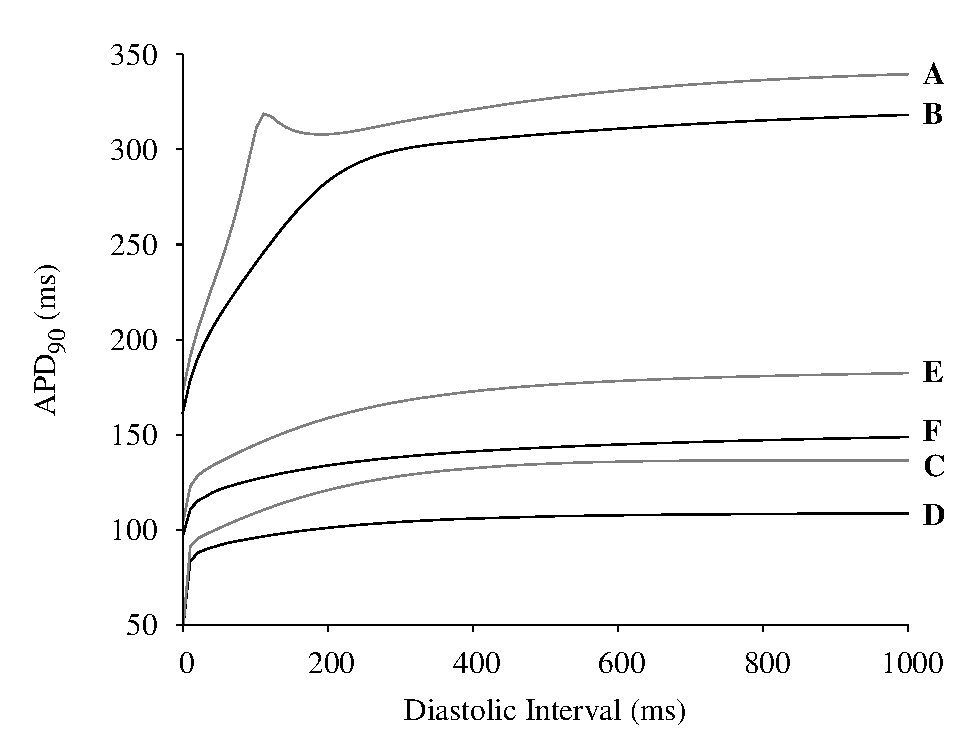
\includegraphics{figures/2_apdr}
\caption{APDr curves for control CT (A), control AM/PM (B), AF1 CT (C),
AF1 AM/PM (D), AF2 CT (E), AF2 AM/PM (F). In all cases the CT action
potentials are above the AM/PM action potentials over the whole of the
range considered.}
\label{fig:apdr}
\end{figure}

In AF tissue, the ERP\emph{r} was flattened for all tissue types compared with
the control cells, as shown in Figure~\ref{fig:erpr}.  The curves also extended
to lower BCLs for AF tissue, indicating that it was possible to excite AF tissue
successfully at a higher rate than was possible in control tissue.
Heterogeneity in ERP\emph{r} was largely unaffected by AF.

\begin{figure}[tb]
\centering
%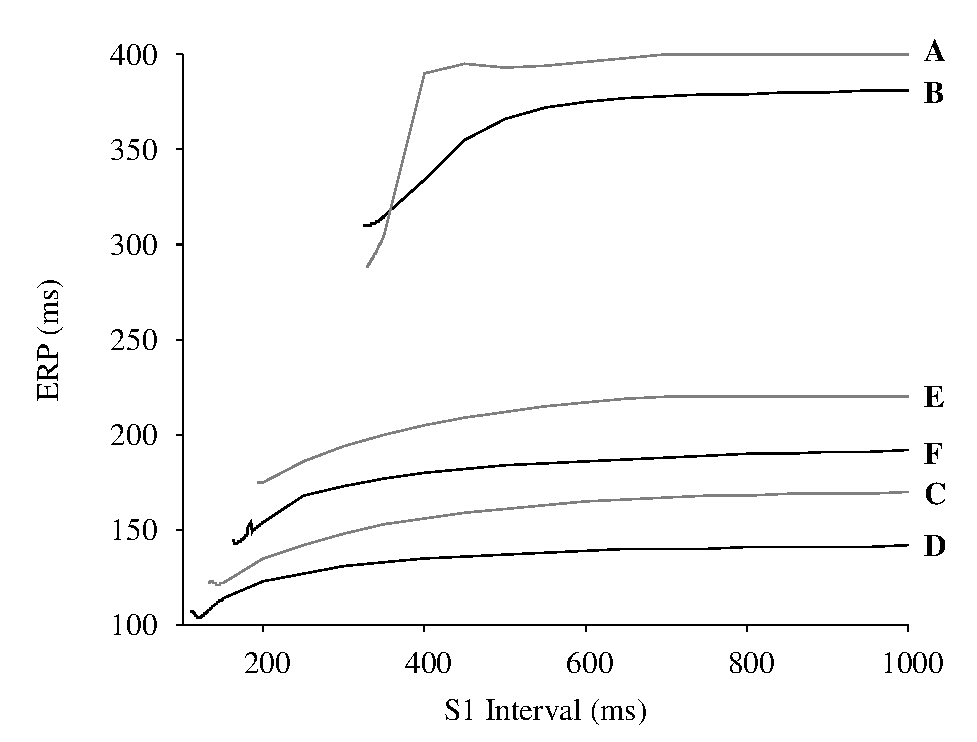
\includegraphics{figures/3_erpr}
\caption{ERPr curves for control CT (A), control AM/PM (B), AF1 CT (C),
AF1 AM/PM (D), AF2 CT (E), AF2 AM/PM (F).  Both AF1 and AF2 have a
significantly reduced ERPr over the whole range considered, with AF1
having a lower ERP then AF2.  In addition, AF1 and AF2 cells are still
excitable after pacing at \ms{100} shorter BCL.}
\label{fig:erpr}
\end{figure}

Conduction velocity, shown in Figure~\ref{fig:cvr}, was slowed by AF,
reducing the solitary wave velocity from $0.27\,\text{mm}\,\text{ms}^{\text{-1}}$\ in
control to $0.25\,\text{mm}\,\text{ms}^{\text{-1}}$\ in AF1 and
$0.26\,\text{mm}\,\text{ms}^{\text{-1}}$\ in
AF2.  Maximal pacing rate increased from the control value of \unit{198}{bpm} to
\unit{421}{bpm} in AF1 strands and \unit{315}{bpm} in AF2 strands.

The VW was reduced by AF, but in all cell types the reduction was small.
The control value of \ms{16.6} was reduced to \ms{14.2} in AF1 and \ms{14.7}
in AF2 for AM and PM cell types.  The reduction in VW for CT cells was
even smaller, from \ms{15.1} in control to \ms{14.5} and \ms{14.4} in AF1 and
AF2, respectively.

\begin{figure}[tb]
\centering
%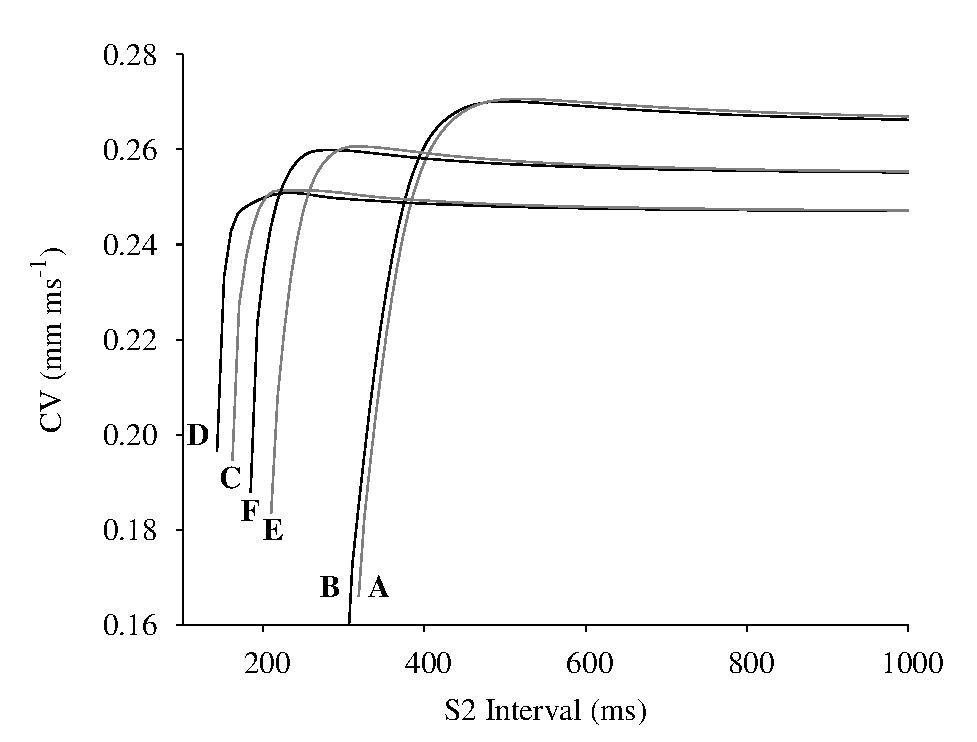
\includegraphics{figures/4_cvr}
\caption{CVr curves for control CT (A), control AM/PM (B), AF1 CT (C),
AF1 AM/PM (D), AF2 CT (E), AF2 AM/PM (F).  In each of the conditions,
the CT cells showed a higher CV at long (1000~ms) S2 intervals, but AM
and PM cells allow faster conduction at shorter S2 intervals.  The AF
cases show reduced CV compared to the control and support a higher
pacing rate via reduced minimum interval.}
\label{fig:cvr}
\end{figure}

Simulations over the 2D geometry examined the lifetime and behavior of
spiral waves in the presence and absence of electrical heterogeneity.
As can be seen in Figure~\ref{fig:plots}, panels Ai and Bi, re-entrant
activity self-terminated in both homogeneous and heterogeneous cases
when due to spiral wave meander over a large tissue region, it
exits the tissue.  Self-termination was much more rapid in the
electrically heterogeneous case, taking \unit{1.31}{s}, compared with
\unit{3.20}{s} in
the homogeneous case.

Conversely, under AF conditions the re-entry persisted after it was
induced for the whole period of the simulation, a lifespan of over \unit{5}{s}.
Under electrically homogeneous conditions, panels Aii and Aiii show a
stable mother rotor rotating anti-clockwise in the tissue.  But in
heterogeneous conditions, as shown in panels Bii and Biii, a similar
mother rotor to the homogeneous cases is visible towards the right of
each frame.  On the left of the frames, the rotor breaks up into
multiple fibrillatory wavelets on the border of the heterogeneous
regions, forming a complex and chaotic pattern of excitation.

\begin{figure*}[t]
\centering
%\includegraphics{figures/figure4}
\caption{Simulation of re-entry in 2D sheets of electrically homogeneous
(A) and electrically heterogeneous (B) sheets.  Columns show
representative frames after initiation of re-entry at t = 0.  Panels i
show data under control conditions, panels ii under AF1 conditions and
panels iii under AF2 conditions.  Re-entry self-terminated under control
conditions in both homogeneous (Ai) and heterogeneous (Bi).  Under AF
conditions, re-entry becomes a sustained mother rotor in
electrically homogeneous conditions (Aii, Aiii).  However, under
electrically heterogeneous conditions AF causes re-entry to degenerate
into erratic propagations on the borders of the heterogeneity (Bii,
Biii).}
\label{fig:plots}
\end{figure*}

\subsubsection{Discussion and conclusions}

AFER induces significant changes in the cellular electrophysiology that
appear to affect rate dependent electrical activities.  It helps to
sustain re-entry, providing evidence to substantiate the hypothesis of
``AF begets AF''.

Considering first the single cell results, one of the most obvious
effects is the striking reduction in the \apd\ and repolarization
properties.  AFER abbreviated \apd\ in AM cells by 66~\% in AF1 and
53~\% in AF2.  Other work has already suggested why the increases shown
in the maximal slope of the APDr can be
pro-arrhythmic~\cite{ByungSoo2002}, as can the reduced
ERP~\cite{Xie2002}.  Our study suggested that reduction is not uniform
across all cell types, which leads to an augmented heterogeneity.

The 1D strand results for the CV tell a similar story.  AFER tissue
forms a much better substrate for arrhythmic activity, supporting both a
much higher maximal pacing rate and in addition, the reduction in
conduction wavelength, to below half the control values. This allows a
greater number of excitation waves to exist in the tissue at any one
time.

The 2D simulations in the realistic sheet show a marked difference in
re-entrant behavior between homogeneous and heterogeneous simulations.
The homogeneous sheets show self-termination of re-entry in control
tissue, whilst the reduced ERP and conduction wavelength allow the rotor
to remain stable and persist for the duration of the simulation in AFER
condtions.  The heterogeneous sheet simulations, show spiral wave
breakup, as observed in real tissue \cite{Kumagai1997}, in both control
and AF simulations, possibly due to elevated plateau potentials and
increased refractory period of the CT cells.  Self-termination is still
observed in control simulations and is more rapid than in homogeneous
tissue.

It is still unclear about the pro- or anti-arrhythmogenic effects of
electrical heterogeneity in the human atria.  Self-termination is more
rapid in the heterogeneous tissue for the control case, but despite AFER
increasing the heterogeneity between tissue types, it doesn't lead to
self termination of the re-entry.  In fact, it leads to breakup of the
spiral wave in the region of the heterogeneity, leading to a region of
erratic propagations, as has been seen in experiment~\cite{Kumagai1997}.
Further study, in both 3D geometries and physiological experiments,
would be needed to elucidate the true effects of the heterogeneity.



    \chapter{Modelling the Whole Atrium}

In the previous chapter a modelling library suitable for simulation of single
cell and over 1D and 2D models of cardiac tissue was developed.
Single cell models are the base on which 1D and 2D models stand and 1D and 2D
models provide valuable insight into the behaviours of cardiac tissue in health
and disease.
It does not need to be said that the atrium is not 1D or 2D construct but is
instead a complex 3D structure.
This complexity can be seen internally, in that the atrium is comprised of several
separate tissue types with distinct electrophysiological behaviours and has
regions of differing conductivity.
It can also be seen in the gross physical structure, the atrium has a complex
topology with both holes for the venous and arterial openings, as well as
openings for the valves.
The simpler, often idealized, models constructed in the previous chapter
ignore (and in many cases, are incapable of showing) many of these complexities.
To provide insight into the atrium function on the whole organ level we must
therefore simulate the atrium as an organ.
A 3D model of the atrium requires a representation of the atrial geometry to
provide the topology of the atrium.
To model complexities with sufficient accuracy models of the
electrophysiologically distinct tissue types are also required as are
descriptions of the complex conductivities.


\section{Atrial Geometry}
\label{atrium:sec:geometry}

The atrial geometry used in the simulation studies presented here was based on
the visible human project female dataset.  The visible human dataset was
created from a pair of cadavers, set into wax and sliced into \mm{1}\ and
\mm{0.33}\ for the male and female bodies, respectively.  The geometric model
used here was extracted from the female dataset and so has a resolution of
\mm{0.33}.  The extracted geometry is segmented into different tissue types,
with distinct classifications for left and right atrium, the pectinate muscles,
the crista terminalis, the Bachmann bundle and the sino-atrial node, as shown in
figure \ref{atrium:geometry}.  The geometry has been used in numerous previous
simulation studies.  It was discretised via a finite differences approach, which
allows the whole atrium to be embedded in a block of $298\times269\times235$
nodes.  This gives it a total size of approximately 19 million total nodes,
although only approximately 1.6 million of those nodes correspond to excitable
cells.  The geometry also has simple fibre orientation in the pectinate muscles,
crista terminalis and Bachmann bundle.  The fibres are considered to always run
parallel to the local axis of the tissue bundle, as determined by principle
component analysis~\cite{Seemann2006}.

\section{Simulation Methods}
\label{atrium:sec:model}

\subsection{Atrial Model}

The electrical activity at each of the nodes was described by the equations of
the Courtemanche--Ramirez--Nattel (CRN) of the human atrial
myocyte~\cite{crn98}.  This model, as previously described, is a second
generation model. It has 21 state parameters, representing ionic gating activations
and inactivations and intracellular concentrations of ionic species.  In the
model, the total current, \ii{ion} is made up of the contributions of numerous
channels
\begin{equation}
\label{atrium:crn}
\ii{ion} = \ii{Na} + \ii{K1} + \ii{to} + \ii{Kur} + \ii{Ks} + \ii{Kr} +
\ii{Ca,L} + \ii{p,Ca} + \ii{NaK} + \ii{NaCa} + \ii{b,Na} + \ii{b,Ca}
\end{equation}
where \ii{Na}, \ii{K1}, \ii{to}, \ii{Kur}, \ii{Ks}, \ii{Kr}, \ii{Ca,L},
\ii{p,Ca}, \ii{b,Na} and \ii{b,Ca}\ represent ionic currents and \ii{NaK}\ and
\ii{NaCa}\ are ion exchangers.  As a second generation model, the CRN model also
has a detailed calcium handling system which can influence the action potential
via its influence on the intracellular calcium concentration.

In some atrial simulations it was desirable to incorporate details of
electrophysiological heterogeneity to represent the difference in electrical
behaviour between atrial myocytes and the other cellular types present in the
geometry, the pectinate muscles and crista terminalis.  The parameters used for
heterogeneity were based on measurements taken by Feng et al.~\cite{feng1998}
of the canine atrium.  These were converted to parameters for the CRN model by
Seemann et al.~\cite{Seemann2004} and have been used in several simulation
studies~\cite{Seemann2006,Stott2008}.  They are shown in
table~\ref{atrium:het_params}.

\subsection{Monodomain Equation}

To simulate the propagation of electrical activity over the finite difference
geometry previously described, the mono-domain equation is used to describe the
changes in $V$ in time, $t$, the trans-membrane voltage.
\begin{equation}
\label{atrium:monodomain}
\frac{\partial V}{\partial t} = \nabla\cdot D \nabla V - \frac{\ii{ion}}{C_{m}}
\end{equation}
where $D$ is a tensor representing the diffusivity of electrical potential, \ii{ion} is described by the
CRN model (\ref{atrium:crn}), $C_{m}$ is the membrane capacitance and all other
symbols have their usual meanings.  Equation (\ref{atrium:monodomain}) is
advanced in time via the forward euler method with a timestep of \ms{0.05}.  For
simulations with isotropic conductivity between nodes a 7-node approximation of
the differential operator is used.  When anisoptropy is present, a 27-node
approximation is used.

\subsection{Tissue Anisotropy}

The heart has a complex fibrous structure (Chapter 1), and this manifests
electrically as regions which have preferential conduction directions.
The preferential conduction directions show greatly increased conduction
velocities, sometimes by a factor of up to five~\cite{}.
The fibre structure and regions of preferential conduction are generally
considered much more important for the ventricles than for the atria.
The atria, or more specifically the right atrium, do possess several structures
with a definite direction of preferential conduction.
These are the crista terminalis, responsible for rapid conduction of the
depolarization wave to the atrio-ventricular node, the pectinate muscles and the
Bachmann bundle, the preferential pathway for conduction between the atria.
To determine the influence of anisotropic conduction on the propagation of the
electrical activity, we follow a method after Panfilov and
Keener~\cite{panfilov1995}.
In this method there is a unit vector, $\mathbf{f}$, defined at every point in
the tissue which has significant fibre orientation.
This unit vector defines a set of co-ordinate axes, in which the conductivity
tensor is diagonal
\begin{equation}
\label{atrium:dtilde}
\mathbf{\tilde{D}} =
\begin{pmatrix}
D_{\parallel} & 0 & 0\\
0 & D_{\perp} & 0\\
0 & 0 & D_{\perp}
\end{pmatrix}
\end{equation}
where $D_{\parallel}$ is the diffusion constant for conduction parallel to the
preferential direction of conduction and $D_{\perp}$ is the diffusion constant
for conduction perpendicular to this direction.
In this formulation it is assumed that there is no `sheet' structure which gives
a higher conduction velocity in one direction perpendicular to the main fibre
axis.
The diffusion tensor $\mathbf{\tilde{D}}$\ will only be diagonal in the
Cartesian co-ordinate system of the heart if the direction of preferential
conduction is parallel to one of the axes.
Therefore, to find the conductivity tensor in the global co-ordinate system,
$\mathbf{D}$, we need to find two transformation matrices $\mathbf{A}$\ and
$\mathbf{A^{T}}$\ such that
\begin{equation}
\label{atrium:d}
\mathbf{D} = \mathbf{A} \mathbf{\tilde{D}} \mathbf{A^{T}}
\end{equation}
To find $\mathbf{A}$\ it is possible to write out the involved rotations
explicitly, however an alternative method~\cite{fention2005}\ uses the fact that
$\mathbf{f}$\ and the two vectors orthogonal to it, $\mathbf{g}$\ and
$\mathbf{h}$\ are eigenvectors of $\mathbf{D}$.
These have the eigenvalues of $D_{\parallel}$\ and $D_{\perp}$.
The matrix $\mathbf{A}$\ is therefore an orthogonal matrix of the form
$\mathbf{A} = \left(\mathbf{f},\mathbf{g},\mathbf{h}\right)$ and so, using
(\ref{atrium:d}) $\mathbf{D}$\ can be written as
\begin{equation}
\label{atrium:dfgh}
\mathbf{D} = D_{\parallel}\mathbf{f}\mathbf{f^{T}} +
D_{\perp}\left(\mathbf{g}\mathbf{g^{T}} + \mathbf{h}\mathbf{h^{T}}\right)
\end{equation}
Using the fact that $\mathbf{A}\mathbf{A^T} = \mathbf{I}$ it is possible to
write
\begin{equation}
\label{atrium:dwithf}
\mathbf{D} = D_{\perp}\mathbf{I} + \left(D_{\parallel}-D_{\perp}\right)\mathbf{f}\mathbf{f^{T}}
\end{equation}
where $\mathbf{I}$\ is the identity matrix, and all other symbols are as defined
previously.
The directions of preferential conduction for the atrial geometry used in the
study were described by a pair of angles $\theta$\ and $\phi$\ representing the
orientation of the unit vector $\mathbf{f}$\ at each point in spherical polar
co-ordinates.
In cells with no assigned preferential conduction direction, the components of
$\mathbf{f}$\ were set to zero, giving a diffusion tensor of
\begin{equation}
\label{atrium:dnofibre}
\mathbf{D} =
\begin{pmatrix}
D_{\perp} & 0 & 0\\
0 & D_{\perp} & 0\\
0 & 0 & D_{\perp}
\end{pmatrix}
\end{equation}
which is the diffusion tensor for isotropic conduction.

\subsection{Computational Implementation}

The atrial geometry used in these studies is quite large, consisting of almost
19 million nodes.
As noted in \ref{atrium:sec:geometry}, only approximately 1.6 million of these
nodes correspond to active tissue--less than 10\% of the total.
The electrical activity at each node is represented by the CRN model and thus
requires 21 double precision numbers to be stored, representing the state
variables of the model.
The memory requirements of the model may be significantly reduced by storing
state variables, and where anisotropy is present the diffusion tensor, only for
the active nodes.
This reduces the memory requirements for storing the state variables from
approximately \unit{2.9}{GB}\ to \unit{256}{MB}.
A further simplification may be obtained by decomposing the geometry into a
linear array, containing the 7 or 27 neighbours of the active nodes to be used
in the diffusion tensor approximation.
The geometry and state information can therefore be represented by one linear
array of cellular states, one linear array used as a `map' and optionally, one
linear array representing the components of $\mathbf{D}$.
This linear data structure is very easy to parallelize on a shared memory
system.

The parallelization was accomplished through the use of the OpenMP shared
memory parallelism library~\cite{OpenMP}.
The system was then solved on 1 node of the Horace supercomputer on a total of 8
cores.
The linear array of active nodes was divided equally between the 8 cores, with
each core solving (\ref{atrium:crn}) for all nodes its assigned section of the
array.
A snapshot of the trans-membrane potentials at each of the active node sites was
output every \ms{2.5}\ of simulated time.
Simulation of \unit{1}{s}\ of atrial activity took XXXX hours.
A parallel fraction of XXXX was attained, indicating that almost all of the
workload was effectively distributed over the 8 cores.

\section{Mutation in KCNQ1: A Simulation Study}

Atrial Fibrillation (AF) is the most common arrhythmia in the developed world.
It is a self-promoting condition, with paroxysmal AF episodes frequently
degenerating into chronic and even permanent AF.
Clinically, AF patients show an erratic and high frequency ECG.
At the cellular level, AF is characterised by an abbreviated action potential
(AP) which has no plateau phase and poor heart rate adaptability.
The mechanisms through which AF influences the heart are complex, but the
remodelling of the cellular electrophysiology is believed to contribute to
reduced ERPs and through that, favour the formation of stable, long lived
spiral waves and organ level microwavelet re-entry.
AF is often preceeded by congestive heart failure, cardiomegaly and other
structural cardiac diseases, but there are significant numbers of suffers with
no such structural defects.
There is also evidence of a genetic predisposition to AF, which is sometimes
termed Familial Atrial Fibrillation.
Several gene mutations have been causally implicated for AF, leading to AF
which manifests both with and without associated structural cardiac disorders.
The ion channels associated with the repolarisation reserve (\ii{K1}, \ii{Kr},
\ii{Ks}) are particularly important to the genesis of AF.
Alterations in functions, gating and kinetics have been implicated in both short
and long QT syndromes.
The \ii{Ks}\ channel has very slow activation kinetics which enable it to
regulate cardiac APs over a wide range of plateau voltages.
Mutations in the \ii{Ks}\ channel are common.
Several mutations in the $\alpha$-subunit, coded for by the KCNQ1 gene, of the
\ii{Ks}\ channel have been identified including both loss-of-function and
gain-of-function, leading to the SQT syndrome and to AF.
Chen et al. studied a four generation Chinese family with hereditary persistent
AF.
They identified a missense mutation at nucleotide 418 from adenine to guanine
resulting in a change from serine to glycine at position 140 (S140G mutation of
\ii{Ks}).
This missense mutation lead to a large gain-of-function which included changes
in the channel kinetics.
It has been hypothesised that these changes in the function of the \ii{Ks}\
channel in the human atrium result in abbreviations of both APD and ERP and thus
provide an appropriate substrate for the genesis of AF.

This study had two goals: To construct a computer model of the available
experimental data from Chen et al. and to then use this model to quantify the
effects of the mutation through the use of cellular, 1D, 2D and 3D models

\subsubsection{Modelling the Mutation}

This study, as in the previous chapter, uses the CRN model, developed by
Courtemanche et al.~\cite{CRN1998}\ for simulation of the human atrial action
potential.
As a biophysically detailed model with 21 state variables and numerous ion
channels it is ideal for use in mutation studies.
The CRN model has individual descriptions of several $K^{+}$\ currents.
These include the time-independent potassium current, \ii{K1}, the ultra-rapid
potassium current, \ii{Kur}, the transient outward current, \ii{to}\ and the
rapid and slow delayed rectifier currents, \ii{Kr}\ and \ii{Ks}.
The latter current is modulated by the mutation and is described in the control
CRN cell by
\begin{equation}
\label{atrium:iks_con}
\ii{Ks} = g_{Ks}x_{s}^{2}\left(V-E_{K}\right)
\end{equation}
where $g_{\tiny{Ks}}$\ is the channel conductance (\unit{0.129}{nS/pF}), $x_{s}$\ is
the activation variable and $E_{K}$\ is the $K^{+}$\ reversal potential, found
through the Nernst potential.

\subsubsection{Simulation of the S140G mutation of KCNQ1 I-V relationship}

The Chen et al.~\cite{Chen2003} study determined that the most likely cause of
familial AF was was the S140G mutation of the KCQN1 gene, which forms part of
the $\alpha$-subunit of the \ii{Ks}\ channel.
The gene was transfected into COS7 cells along with the second component of
the $\alpha$-subunit, KCNE1, in both normal (WT) and mutated type (MT).
The transfected cells were used to perform voltage clamp experiments.
The clamp protocol used is shown in Figure~\ref{atrium:iks:vc},A.
This is the experimental protocol used by Chen et al.~\cite{Chen2003}.
The cell was held at a holding potential of \mv{80} for \unit{0.5}{s}\ before
being held at \mv{10}\ steps between \mv{-130}\ to \mv{50}\ for \unit{3}{s}.
The voltage steps were followed by a \mv{-40}\ holding potential, applied for
\unit{1}{s}.
The values of \ii{Ks} at the end of the step voltages were plotted against the
step voltages to determine  I-V relationships for WT
and MT cells, shown in Figure~\ref{atrium:iks:vc},B (points with errors) and
current traces, shown in Figure~\ref{atrium:iks:vc},C and D for WT and MT,
respectively.

\begin{figure}
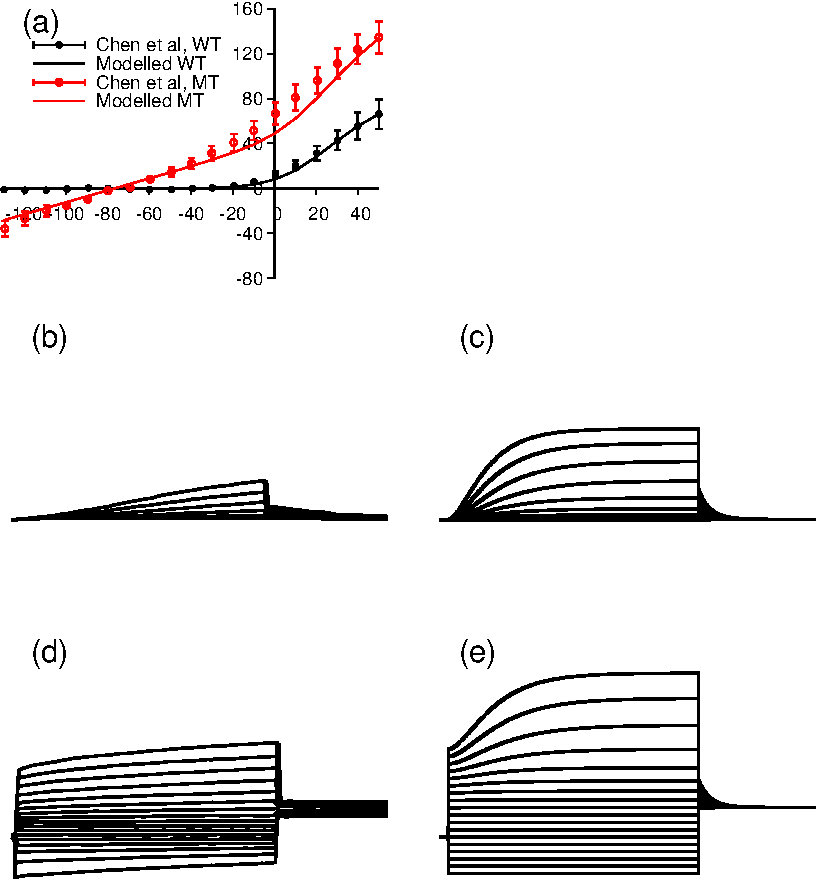
\includegraphics{figures/atrium/iks/figures/01_IV}
\caption[KCNQ1 mutation in IKs, experimental data]{
\label{atrium:iks:vc}
\textbf{A} Voltage clamp protocol used by Chen et al.~\cite{Chen2003}.
\textbf{B} Experimental WT (black, closed circles) and MT (red, open circles)
I-V relationships recorded by Chen et al.  Simulated I-V curves for WT (black
lines) and MT (red lines).  Modelled curves are scaled to experimental points
based on the WT current density at \mv{50}.
\textbf{C} Experimental current traces for WT.
\textbf{D} Simulated current traces for WT.
\textbf{E} Experimental current traces for MT.  Note the instantaneous
activation, and the significant inward current at negative clamp potentials.
\textbf{F} Simulated current traces for MT.
}
\end{figure}

The I-V relationship shows that the mutation causes a gain-of-function across
all the clamp potentials.
It also reveals that the mutation appears to cause an inward current at negative
potentials.
The current traces suggest a drastic change in the kinetics of the \ii{Ks}\
channel with a significant component of the current being activated immediately.
The addition of a leakage component to (\ref{atrium:iks_con}) allowed simulation
of \ii{Ks}\ characteristics which closely matched the experimental data.
Under MT conditions, the new total current \iip{Ks}\ was described by
\begin{equation}
\label{atrium:iks_mut}
\iip{Ks} = \ii{Ks} + \varphi g_{Ks}x\left(V-E_{rev}\right)
\end{equation}
where \ii{Ks}\ is (\ref{atrium:iks_con}), $\varphi$\ is a multiplicative parameter
from with values between 0 and 1, $g_{Ks}$ is as in (\ref{atrium:iks_con}) and
$E_{rev}$\ is the reversal potential of the leakage component.
The reversal potential was estimated from the experimental I-V relationships to be
\mv{-76.3}.
The inclusion of the $\varphi$\ parameter allowed the simulation of several
intermediate mutant states, representative of a heterozygous mutation.
Setting $\varphi = 1$\ and following the voltage clamp protocol shown in panel A
of Figure~\ref{atrium:iks:vc}\ the I-V relationship of \ii{Ks}\ was simulated to
provide a good match to experimental data shown as the lines in panel B of
Figure~\ref{atrium:iks:vc}.
Also shown are the simulated current traces elicited by the voltage clamp
protocol in panels D and F.
The non-gated leakage component of \iip{Ks}\ sufficiently accounts for the
changed current density and kinetics.

\subsubsection{Simulation Protocols}

To assess the effects of the mutation on human atrial myocytes, cellular models
including the modified \iip{Ks}\ described by (\ref{atrium:iks_mut}) were used
in a number of simulation protocols, as described in Chapter 2.
Initially the \apd\ was evaluated under conditions corresponding to $\varphi =
0$\ (WT) and $\varphi = 1$\ (MT).
Under such conditions, the induced \apd\ shortening was found to result in
un-physiological \apd\ values, shown in Figure \ref{atrium:iks:apd}.
Therefore a pair of heterozygous cases, corresponding to $\varphi = 0.10$\
(HT10) and $\varphi = 0.25$\ (HT25) were created and used in the evaluation of
the mutation's effects.

Using the models and protocols described in Chapter 2 the \apdr, ERP\emph{r}, VW,
CV\emph{r}, SVW and the dynamic behaviours of spiral waves were evaluated for
the WT, HT10 and HT25 cases.
For the 3D simulations, the model described in Sections
\ref{atrium:sec:geometry}\ and \ref{atrium:sec:model}\ was used.
Since the intention was just to investigate the influence of the mutation, the
model was used without tissue anisotropy.
The mutation was applied homogeneously with the electrical activity at all
nodes described by either the WT or HT10 cells.
An atrial model of nodes described by HT25 cells did support stable conduction
and so it was not used in the 3D studies.
There was no heterogeneity introduced to account for the differing cell types
present in the human atrium.
To examine the behaviour of scroll waves under WT and HT10 conditions a protocol
analogous to the wave-break protocol described for 2D sheets of tissue was
used~\cite{Kharche2007}.
The protocol is illustrated in Figure~\ref{atrium:iks:scroll_init}.
\begin{figure}
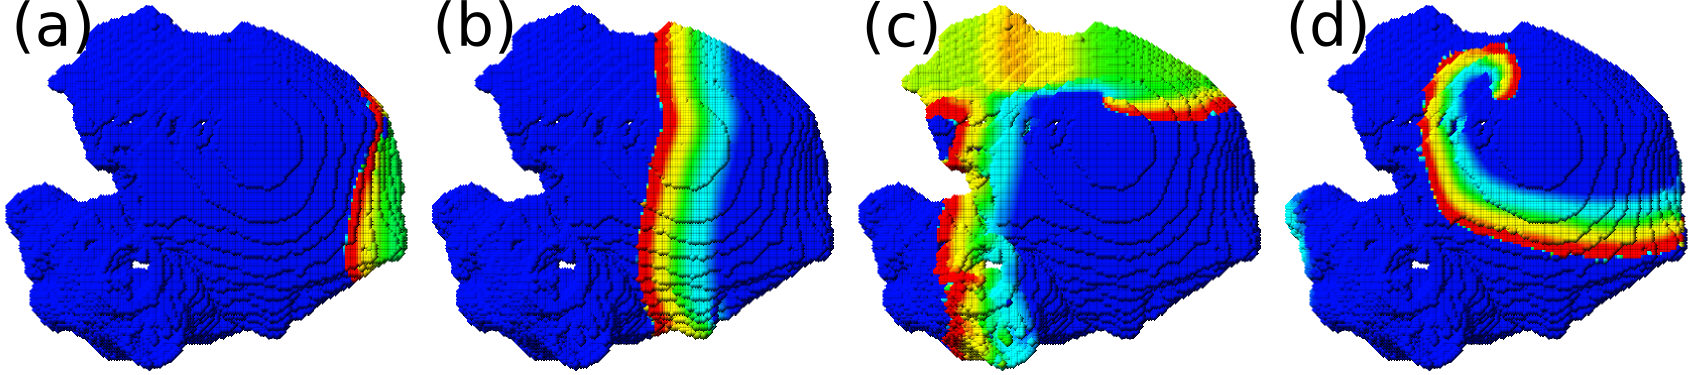
\includegraphics{figures/atrium/iks/scrollhowto}
\caption[Initiating a Scroll Wave]{
\label{atrium:iks:scroll_init}
Stimulus protocol used to initiate a scroll wave.
\textbf{A} One extreme of the atrial model is stimulated
\textbf{B} The excitation is allowed to propagate
\textbf{C} An S2 stimulus is delivered by clamping a section of the tissue, here
the lower quarter.
\textbf{D} A scroll wave begins on the wall of the right atrium.
}
\end{figure}
First, a small number of cells are simulated at one extreme of the atrial model.
The excitation is allowed to propagate through the model until the S2 stimulus
is delivered.
The S2 stimulus is delivered via briefly clamping a section of the atrial model to
\mv{50}\ and then releasing the clamp.
A correctly timed S2 stimulus results in a scroll wave on the wall of the right
atrium.
After initiation, the models were simulated until activity ceased or until
\unit{6}{s}\ of simulated time had elapsed.

\subsubsection{Changes in \apd\ due to S140G mutation}

The effect of an increase in the leakage current parameter were investigated.
This was done using the standard \apd\ protocol and varying $\varphi$\ between
0 and 1.
Variation in \apd\ as $\varphi$\ is altered is shown in
Figure~\ref{atrium:iks:aps},A.
Representative APs are shown in Figure~\ref{atrium:iks:aps},B.
The \apd\ under Control conditions (WT) was seen to be \ms{312.0}.
Progressive mutation decreased the \apd\ to \ms{150.5}\ in HT10 case and
\ms{79.3}\ in HT25 case.
Under homozygous conditions, $\varphi = 1$\, the \apd\ was seen to be \ms{22.4}.
Figure~\ref{atrium:iks:aps},B shows the inclusion of the mutant channel causes
the changes in morphology associated with none of the mutant types having a
plateau region.
Inclusion of the mutant channel decreased the upstroke velocity of the AP from
\unit{217.1}{V/s}\ in WT, to \unit{214.0}{V/s}\ in HT10 and \unit{208.6}{V/s}\
in HT25.
The upstroke velocity in the homozygous case was \unit{192.0}{V/s}.

\subsubsection{\apdr\, ERP\emph{r}, CV\emph{r} and VW}

Figure~\ref{atrium:iks:apdretal},A shows the current profiles of \ii{Ks} over the course of
an AP which correspond to the AP traces shown in Figure~\ref{atrium:iks:aps},B.
\ii{Ks}\ is seen to increase considerably in both the HT10 and HT25 cases
compared with the WT case.
The leak also changes the morphology of the current profile to one showing
almost instant activation in HT10 and HT25 cases, compared to the slow
activation in WT.
The \apdr\, Figure~\ref{atrium:iks:apdretal},B, reflects the decreased \apd\ with
the restitution curves considerably flattened for both the mutant cases.
The maximal slopes of the \apdr\ were measured to be 1.9, 0.78 and 0.56 in cases
WT, HT10 and HT25 respectively.
The ERP\emph{r}\ curves, Figure~\ref{atrium:iks:apdretal},C, also reflect the
reduced \apd\.
At an S1 interval of \ms{1000}\ the ERP was found to be \ms{XXXX}\ in WT,
\ms{XXXX} in HT10 and \ms{XXXX} in HT25.
In addition, the mutant cases supported excitation at much lower S1 intervals
(or higher pacing rate) compared to the control case.
The minimum S1 interval sustained during the ERP\emph{r}\ calculations was
\ms{XXXX}\ in WT, \ms{XXXX} in HT10 and \ms{XXXX} in HT25.
The solitary wave CV was not altered considerably by the mutation (\cms{26.7}\
in WT c.f. \cms{27.0} in HT25).
The CV\emph{r}\, Figure~\ref{atrium:iks:apdretal},D, curves confirm the findings
of the ERP\emph{r}\ calculations, that the mutant case supports successful
excitation after a considerably reduced S2 interval.
The minimum S2 interval which still allowed the test stimulus to propagate was
found to be \ms{318.9}\ in WT, \ms{181.2}\ in HT10 and \ms{120.4}\ in HT25.
Vulnerability to premature excitation was relatively unaffected by the mutation,
having a value of approximately \ms{XXXX} in all cases.


    \bibliography{refs}

\end{document}
